\UseRawInputEncoding
%% Proxy4Tun — Automation in Construction (cas-dc double-column template)
%% Merged publication draft, 15 Sep 2026.
%% Structure and framing follow main.tex; methodology, results, and appendices
%% follow Proxy4Tun_journal_publish-2026-09-15.tex (four-feature proxy,
%% 54-run stress test, 22-case four-arm refinement panel).

\documentclass[a4paper,fleqn]{cas-dc}

\usepackage[numbers]{natbib}
\usepackage{booktabs}
\usepackage{array}
\newcolumntype{Y}[1]{>{\raggedright\arraybackslash}p{#1}}
\usepackage{multirow}
\usepackage{amsmath}
\usepackage{algorithm}
\usepackage{algpseudocode}
\usepackage{graphicx}
\usepackage[dvipsnames,table]{xcolor}
\usepackage{xurl}
\usepackage{hyperref}
\usepackage[nameinlink,noabbrev]{cleveref}
\usepackage{placeins}
\usepackage{caption}
\usepackage{float}
\usepackage{tikz}
\usetikzlibrary{shapes.geometric,arrows.meta,positioning,fit,calc}
\usepackage{listings}
\lstset{
  basicstyle=\ttfamily\footnotesize,
  breaklines=true,
  columns=fullflexible,
  frame=single,
  framesep=4pt,
  xleftmargin=0.5em,
  xrightmargin=0.5em,
  aboveskip=0.6em,
  belowskip=0.6em,
}

\providecommand{\printorcid}{}
\providecommand{\printfacebook}{}
\providecommand{\printtwitter}{}
\providecommand{\printlinkedin}{}
\providecommand{\printgplus}{}
\providecommand{\printinstagram}{}
\providecommand{\printemails}{}
\providecommand{\printurls}{}

\begin{document}
\let\WriteBookmarks\relax
\def\floatpagepagefraction{1}
\def\textpagefraction{.001}

% ────────────────────────────── Front matter ──────────────────────────────

\shorttitle{Proxy4Tun: proxy-driven quality control for point-cloud tunnel-lining segmentation}
\shortauthors{X.\ Tao et~al.}

\title[mode=title]{\texorpdfstring{Proxy4Tun: proxy-driven quality control for point-cloud tunnel-lining segmentation}{Proxy4Tun: proxy-driven quality control for point-cloud tunnel-lining segmentation}}

\author[1]{Xinghui Tao}
\credit{Conceptualization, Methodology, Software, Writing -- original draft}

\author[2]{Zehao Ye}

\author[1]{Guangming Wang}
\cormark[1]
\ead{gw462@cam.ac.uk}
\credit{Supervision, Writing -- review \& editing}

\author[2]{Jelena Nini\'{c}}
\credit{Supervision, Writing -- review \& editing}

\author[1]{Brian Sheil}
\credit{Supervision, Funding acquisition, Project administration, Writing -- review \& editing}

\cortext[cor1]{Corresponding author}

\affiliation[1]{organization={Construction Engineering, University of Cambridge},
    addressline={Trumpington Street},
    city={Cambridge},
    postcode={CB2 1PZ},
    country={United Kingdom}}

\affiliation[2]{organization={Department of Engineering, Durham University},
    addressline={Stockton Road},
    city={Durham},
    postcode={DH1 3LE},
    country={United Kingdom}}

% ─── Abstract ─────────────────────────────────────────────────────────────

\begin{abstract}
Tunnel-lining segmentation supports point-cloud inspection, but changing tunnel conditions and scarce reference labels complicate quality assessment of new outputs. Proxy4Tun estimates segmentation accuracy from intermediate pipeline measurements, using one labelled development subset and one expert-tuned reference configuration per lining family. Across three Seg2Tunnel families, bounded space-filling sampling and uncertainty-guided Bayesian exploration produce 120 calibration runs; model comparison and feature ablation identify a four-feature Ridge proxy that predicts mean intersection-over-union (mIoU) without reading GT labels. On 54 paired runs from 27 held-out subsets, the frozen proxy achieves a Spearman correlation of 0.817 and a mean absolute error (MAE) of 0.109, ranks every reference output above its degraded counterpart, and flags all 27 degraded runs with three alarms on reference runs. On 22 cases admitted by the proxy band $[0.5,0.7)$, three LLM proposal systems and a sparsity-matched random-overlay control share one GT-blind selector: mean mIoU rises from 0.738 to 0.751--0.760 (LLMs) and 0.752 (random), whereas unselected random proposals fall to about 0.53. Point-level error analysis attributes the gain to fewer whole-ring class swaps and identifies the proxy's main blind spot: a rotation of block labels between correctly placed joints leaves all four measurements unchanged. Proxy4Tun demonstrates that limited development supervision can be transferred to deployment quality control and bounded parameter refinement, and that proxy-based selection, rather than the proposer, carries most of the observed gain.
\end{abstract}

% ─── Highlights ───────────────────────────────────────────────────────────

\begin{highlights}
\item Proxy4Tun estimates tunnel-segmentation accuracy without deployment labels.
\item Calibration uses one labelled subset and one expert reference per lining family.
\item Frozen four-feature proxy ranks all 27 reference/degraded pairs on unseen scans.
\item One GT-blind selector lifts mIoU 0.738 to 0.751--0.760 for LLM and random proposers.
\item Refinement fixes whole-ring class swaps; pure label rotation escapes the proxy.
\end{highlights}

% ─── Keywords ─────────────────────────────────────────────────────────────
\begin{keywords}
Segmental tunnel lining \sep Point cloud segmentation \sep Deployment quality control \sep Label-free quality estimation \sep Parameter refinement \sep Large language models
\end{keywords}
\date{\today}

\maketitle

% ═════════════════════════════════════════════════════════════════════════
\section{Introduction}
\label{sec:intro}

Regular inspection of segmental tunnel linings supports structural health assessment and long-term operational safety. Large tunnel networks and restricted access make manual inspection resource-intensive, motivating cost-effective data collection and analysis~\cite{attard2018,montero2015,strauss2020sensing}, and laser scanning captures the lining surface as a 3D point cloud quickly enough to make network-scale inspection practical~\cite{huang2021bim,sjolander2023towards,weidner2024generalized}. Most downstream inspection tasks first require assigning each point to its lining block. Segmentation accuracy, however, changes with lining geometry, joint layout, occlusion, and scan quality, and checking every new output against manual labels or re-tuning parameters by hand is a recurring cost. Practitioners therefore need to decide whether an output is accurate enough to accept, should be refined, or must be flagged for human review, without new ground-truth (GT) labels (Fig.~\ref{fig:deployment_qc_gap}).

\begin{figure*}[t]
\centering

\includegraphics[width=0.8\textwidth]{figs/motivation.pdf}
\caption{Deployment quality-control (QC) problem: segmentation methods produce candidate outputs, but practitioners still need to decide whether to accept, refine, or flag each result. Without new GT labels, this decision requires other evidence about segmentation accuracy.}
\label{fig:deployment_qc_gap}
\end{figure*}

Existing segmentation approaches can be compared using two practical deployment questions: (i) how they cope with changing tunnel and scanning conditions, and (ii) what evidence they provide that a specific output is accurate (Fig.~\ref{fig:conceptual_positioning}). Engineer-designed geometric pipelines use hand-crafted rules and thresholds with interpretable checks, but changes in geometry or scan quality can require manual tuning or redesign~\cite{huang2021bim,weidner2024generalized,wang2025automated}. Supervised models can be retrained on labelled data and may provide confidence or uncertainty scores, but these scores must be checked against actual accuracy before they can support QC on new scans~\cite{su2024review,cha2024deep}. Foundation-model pipelines reduce per-project annotation and support adaptation through prompts and preprocessing parameters~\cite{bommasani2021foundation,kirillov2023sam,ye2024sam}. However, the ability to adjust a pipeline does not establish whether the resulting segmentation is better or accurate enough to accept.

Previous studies show that segmentation accuracy can be estimated without GT labels for the new case. In medical imaging, quality estimators learn from labelled development data or assess new outputs through labelled reference collections~\cite{valindria2017rca,robinson2018segmentationQuality,fournel2021segmentationQC}. It remains unclear how well these approaches transfer to tunnel point-cloud pipelines, where annotations are limited and processing depends on engineering reference configurations. This motivates our central research question: \emph{can measurements produced during tunnel segmentation be calibrated using a small labelled subset and an expert-tuned reference configuration per lining family, then used to estimate accuracy and guide parameter refinement on unseen scans without new GT labels?}

\begin{figure*}[t]
\centering

\includegraphics[width=0.9\textwidth]{figs/position.pdf}
\caption{Conceptual positioning by deployment adaptability and deployment QC strength. Adaptability describes how methods adjust to changing conditions; QC strength describes the evidence they provide for deciding whether to accept, refine, or flag individual outputs without new GT labels. Proxy4Tun combines an intrinsic proxy score with proxy-guided parameter refinement. Positions illustrate intended capabilities rather than results from a comparative QC benchmark.}
\label{fig:conceptual_positioning}
\end{figure*}

Proxy4Tun addresses this question by estimating the accuracy of a candidate segmentation from intermediate pipeline measurements. These measurements describe two aspects of the processing: preprocessing quality (PQ), which reflects the completeness and geometric plausibility of the representation supplied to the segmentation stage, and structure coherence (SC), which reflects whether the recovered layout is internally consistent, that is, whether label boundaries agree with detected joint evidence, whether the lining is covered, whether the label ordering is consistent across rings, and whether the detected ring count matches the expected count. During development, we learn how these measurements relate to GT mean mIoU, then freeze the estimator for deployment. Our hypothesis is that parameter changes produce recognisable patterns in these measurements when processing succeeds or fails, and that their relationship with accuracy persists on unseen scans from the same lining family.

Within a pipeline adapted from SAM4Tun~\cite{ye2025sam4tun}, we generate calibration runs using one labelled development subset and one expert-tuned reference configuration per lining family (staggered, continuous, and complex). We first sample settings across prescribed parameter ranges, then use uncertainty-guided Bayesian exploration to select further settings for evaluation; all runs reuse the same scan annotations. We test the resulting estimator on held-out scans and deliberately degraded outputs, and then use it as the only selection signal in a bounded refinement loop in which three LLM proposal systems and a random-overlay control propose parameter changes. The approach is deployment-label-free in the sense that GT labels are required only during development and offline evaluation; the scorer, the selector, and every proposal prompt exclude them. One annotation-derived input remains upstream: the evaluated pipeline reads the dataset's per-point ring index to orient and validate the unfolded coordinate frame (Section~\ref{sec:pipeline}). The paper therefore claims GT-blind scoring and selection, not end-to-end annotation-free execution. In the conceptual map of adaptability versus QC strength (Fig.~\ref{fig:conceptual_positioning}), Proxy4Tun occupies the high-QC, moderate-adaptability region, combining bounded parameter refinement with explicit, label-free accuracy estimation.

In short, Proxy4Tun delivers a frozen four-feature Ridge proxy that ranks held-out reference runs above paired degradations, and a retained-start selector that converts bounded parameter proposals into a modest mean mIoU gain without reading GT at scoring or selection time. The study isolates selection from proposer identity and shows that residual harm is concentrated in whole-ring label rotations to which the proxy is blind.

This paper makes the following contributions:
\begin{enumerate}
\item A deployment-label-free QC framework that learns to estimate tunnel-segmentation accuracy from PQ and SC measurements using limited offline annotations, and that is frozen before any evaluation.
\item An empirical evaluation of which measurements transfer across lining families and whether the frozen estimator distinguishes reference outputs from deliberately degraded counterparts on scans excluded from fitting, with numerical fidelity, pairwise ranking, and alarm performance reported separately.
\item A proxy-guided refinement study with three LLM proposal systems and a sparsity-matched random-overlay control sharing one GT-blind selector, which separates the value of proxy-based selection from the identity of the proposer, together with a point-level error analysis that attributes the gain to corrected whole-ring class swaps and identifies the measurements' blind spot to label rotation.
\end{enumerate}

The rest of this paper is organised as follows. Section~\ref{sec:related} reviews related work. Section~\ref{sec:methods} presents the methodology and experimental design. Section~\ref{sec:results} reports the results, Section~\ref{sec:discussion} discusses findings and limitations, and Section~\ref{sec:conclusions} concludes.

% ═════════════════════════════════════════════════════════════════════════
\section{Related work}
\label{sec:related}

\subsection{Segmentation, adaptation, and quality estimation}

Tunnel point-cloud segmentation methods differ in how they use geometric knowledge and labelled data. Engineer-designed pipelines use geometric rules and thresholds~\cite{huang2021bim,weidner2024generalized,wang2025automated}; supervised methods such as PointNet++, RandLA-Net, Mask3D, and TD3D learn features from labelled clouds~\cite{qi2017pointnet,hu2020randla,schult2023mask3d,kolodiazhnyi2024td3d}; tunnel-specific networks such as LiningNet integrate structural geometry~\cite{lin2025liningnet}. Labelled tunnel data remain limited, and adapting supervised models may require additional annotations~\cite{su2024review,cha2024deep}.

Foundation-model pipelines reduce task-specific training by projecting clouds into images for SAM, SAM2, or SEEM~\cite{kirillov2023sam,ravi2024sam2,zou2023segment}, with infrastructure applications in crack segmentation and Scan-to-BIM~\cite{ge2024cracksam,ye2024sam,wang2024omni,pan2024zero,ye2026maintenance}. SAM4Tun unfolds linings into panoramas and prompts SAM without task-specific training~\cite{ye2025sam4tun}, but its preprocessing and prompting still depend on geometry- and scan-specific parameters. R4Tun uses reference information and an LLM to propose bounded adjustments without GT access~\cite{taoR4Tun}, leaving open how to assess initial and adjusted outputs when new labels are unavailable.

Quality estimators predict accuracy from observable properties: medical imaging predictors of Dice or overlap~\cite{kohlberger2012evaluating,robinson2018segmentationQuality}, LidarMetaSeg for driving scenes~\cite{colling2021lidarmetaseg}, and consistency checks that can still agree on incorrect labels~\cite{bogdoll2025labelfree}. Reference-based approaches such as RCA and ConfIC-RCA avoid GT for the new case but still use labelled references during assessment~\cite{valindria2017rca,cosarinsky2026conficrca}. Proxy4Tun scores a run from its own PQ and SC measurements and an expected ring count, without comparing against reference-run measurements at scoring time.

\subsection{Calibration and feedback-guided refinement}

Training a quality estimator needs examples spanning successful and degraded segmentations; Robinson et al.\ generate multiple segmentations by varying model settings and reuse existing annotations~\cite{robinson2018segmentationQuality}. Bayesian optimisation and space-filling designs guide which settings to evaluate~\cite{souza2020prior,hvarfner2022pibo,joe2008constructing,gramacy2009adaptive,gramacy2020surrogates}. Proxy4Tun explores around an expert reference to learn from both healthy and degraded outcomes rather than to concentrate on high-accuracy settings alone.

LLM agents can revise results through critique and feedback~\cite{madaan2023selfrefine,shinn2023reflexion,novikov2025alphaevolve,zhang2025darwin}, but self-correction without external feedback can fail and an imperfect proxy can be over-optimised~\cite{huang2024selfcorrect,gao2023overoptimization}. Feedback is more useful when it describes what may be wrong~\cite{yao2023react}. Proxy4Tun supplies PQ and SC measurements for diagnosis and a compact linear score for comparing candidates~\cite{rudin2019stop}; retaining the start keeps the proxy score non-decreasing while testing whether an LLM proposer is needed at all once such a selector is in place.

% ═════════════════════════════════════════════════════════════════════════
\section{Methodology}
\label{sec:methods}

Proxy4Tun has two phases (Fig.~\ref{fig:intrinsic_proxy_scoring}). During development, we vary pipeline parameters on labelled scans and learn how PQ and SC measurements relate to segmentation accuracy; the fitted proxy is then frozen. At deployment, the frozen proxy estimates mIoU without new GT labels, admits a run to refinement or not, and ranks the outputs of bounded parameter proposals. We first define the task and pipeline, then describe calibration, the proxy, the refinement loop, and the experimental design.

\begin{figure*}[t]
\centering

\includegraphics[width=\textwidth]{figs/intrinsics.pdf}
\caption{Development and use of the accuracy proxy. Parameter variations generate segmentation outputs with different accuracies. PQ and SC measurements from each run are paired with GT mIoU to train a Ridge proxy. Once frozen, the proxy estimates accuracy on new runs using the four deployment measurements available without GT. The score is an estimate of segmentation accuracy, not a guarantee of correctness.}
\label{fig:intrinsic_proxy_scoring}
\end{figure*}

\subsection{Task definition}
\label{sec:problem-def}

Given a raw point cloud of a tunnel section, the task is to assign each point a positional lining-block class (key block K, adjacent blocks B1/B2, standard blocks A1--A$n$; Fig.~\ref{fig:task}) or background. Seg2Tunnel, the benchmark dataset we use, groups linings into three families (staggered, continuous, and complex)~\cite{lin2024seg2tunnel}. These families differ in ring geometry and acquisition conditions and, most critically for our task, in the key-block layout: ring-to-ring repeating, fixed ring-wise order, and no repeating pattern. A ring holds six blocks in the staggered and continuous families and seven in the complex family; ring membership is recorded but is not part of the semantic metric.

Proxy4Tun assesses a completed segmentation run. Given its intermediate processing outputs and the expected ring count, the proxy estimates the mIoU that would otherwise require comparison with GT labels. The score supports assessment of the current result and comparison with outputs produced by alternative parameter settings on the same scan. At deployment the proxy remains fixed, and GT labels for the new scan are unavailable to both the scorer and the refinement process.

\begin{figure*}[t]
\centering
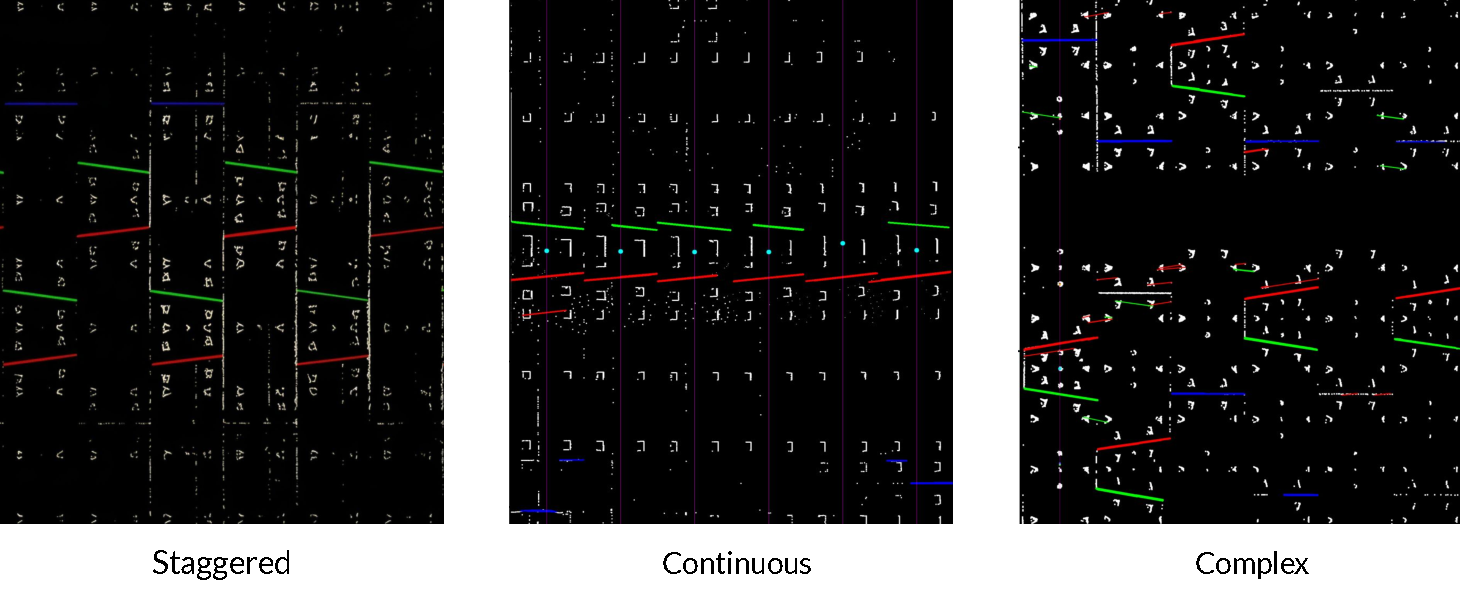
\includegraphics[width=0.8\textwidth]{figs/task.pdf}
\caption{Tunnel-lining block types: key block (K), adjacent block (B), and standard block (A), with background labelled separately. A ring contains six or seven lining blocks depending on its family.}
\label{fig:task}
\end{figure*}

\subsection{Framework overview}
\label{sec:method}

The framework connects three components: a parameterised segmentation pipeline, an offline procedure for learning the mIoU proxy, and a deployment-time refinement loop. The pipeline produces both segmentations and the measurements used to assess them. Calibration learns the relationship between these measurements and GT mIoU. Refinement uses the frozen proxy to compare new candidates. The processing algorithms and SAM weights remain fixed throughout the study; exploration and refinement change only permitted parameter values.

\subsubsection{Segmentation pipeline}
\label{sec:pipeline}

The pipeline is adapted from SAM4Tun~\cite{ye2025sam4tun} for the three Seg2Tunnel lining families. Figure~\ref{fig:pipeline} illustrates the five deployable stages.

\begin{figure*}[t]
\centering

\includegraphics[width=0.98\textwidth]{figs/pipeline.pdf}
\caption{Segmentation pipeline adapted from SAM4Tun. Geometric alignment, filtering, and enhancement produce a depth representation for boundary detection and template-based SAM prompting. The resulting masks are reprojected onto the point cloud. Intermediate outputs provide PQ and SC measurements. The stage algorithms remain fixed; exploration and refinement adjust their parameters.}
\label{fig:pipeline}
\end{figure*}

\begin{enumerate}
\item \textbf{Unfolding.}
RANSAC-based cross-sectional ellipse fitting and centreline estimation establish a cylindrical coordinate system~\cite{fischler1981ransac}. The lining surface is represented panoramically, with depth describing radial distance from the centreline. Coordinate orientation is fixed so that block positions retain the same meaning across runs.

\item \textbf{Denoising.}
Radial masks and grid-based point-density filtering remove points inconsistent with the expected lining surface, following the density-based principle underlying DBSCAN~\cite{ester1996dbscan}. Its settings affect both unwanted-point removal and the amount of lining data retained.

\item \textbf{Enhancement.}
Curvature-guided interpolation and progressive upsampling improve the completeness of the depth representation before detection, while preserving joint boundaries.

\item \textbf{Boundary detection.}
Orientation-specific Hough transforms identify candidate ring and block boundaries~\cite{duda1972hough}. These detections are organised according to the expected family layout.

\item \textbf{Segmentation and reprojection.}
The detected layout defines template-based prompts for SAM~\cite{kirillov2023sam}. The resulting image masks are mapped back to the point cloud to obtain three-dimensional block labels.
\end{enumerate}

A GT-dependent evaluation step runs offline only and has no parameters. Each family has an expert \emph{reference configuration} (\emph{family reference}) that specifies a complete parameter set. A candidate update is an \emph{overlay} listing only the parameters to change; it is applied to an explicitly recorded base configuration, and unchanged parameters retain their base values. Appendix~\ref{app:anchor-parameter} lists the family references and Appendix~\ref{app:bo-config} the exploration bounds, which also define the search space permitted during refinement.

Two conventions matter for what follows. First, stage~1 fixes the coordinate frame using the per-point ring index stored in the Seg2Tunnel files: the centreline direction is chosen so that the axial coordinate correlates with the ring index with a prescribed sign, and the stage aborts unless the Pearson correlation exceeds 0.5 in magnitude. This index is a distributed ring annotation, not sensor metadata. It contributes one binary orientation choice and one validity check per subset, is never passed to the scorer or proposer, and reads no semantic label; but it shapes the frame on which all measurements are computed, so the executed pipeline is annotation-assisted at stage~1 (Appendix~\ref{app:anchor-parameter}). Second, stage-1 parameters are locked during refinement unless the starting run's recentring residual exceeds 10\,cm, so that candidate outputs of one case share a frame.

\subsubsection{Generating calibration examples}
\label{sec:bo-experience}

Calibration requires examples linking observable pipeline measurements to segmentation accuracy under successful and degraded parameter settings. We generate these examples by varying pipeline parameters on one labelled development subset per lining family. All runs on that subset are evaluated against the same annotations, so additional runs require computation but no additional scan labelling.

We collect the examples in two stages (Fig.~\ref{fig:b-p}a). First, scrambled-Sobol sampling provides 32 valid trials spread across the prescribed parameter ranges~\cite{joe2008constructing}; continuous parameters are scaled to their bounds, while discrete parameters are mapped to their permitted values. Second, Bayesian exploration adds eight valid trials at settings whose effects on accuracy remain uncertain. A Gaussian-process (GP) response model with a Mat\'ern kernel ($\nu=2.5$), a white-noise term, and normalised targets learns from the completed evaluations; at each iteration we draw a random pool of 2048 candidate settings within the bounds and evaluate the one with the largest predictive standard deviation, updating the GP after each valid evaluation~\cite{gramacy2009adaptive,gramacy2020surrogates}. This acquisition explores uncertainty in the accuracy response; it does not maximise segmentation accuracy or minimise the final proxy's prediction error, so the records deliberately include poor outputs (GT mIoU from about 0.03 upward).

A trial is valid when all stages complete and all ten candidate measurements are finite; 121 trials were attempted and one failed. Each family contributes 40 valid runs, giving 120 records across the three families. Each record stores its parameter setting, PQ and SC measurements, and GT mIoU. The GP uses parameter settings and GT mIoU to guide exploration, while the accuracy proxy uses PQ and SC measurements to estimate GT mIoU. Algorithm~\ref{alg:bo_exploration} and Appendix~\ref{app:bo-config} give the procedure, sampler and GP configuration, and per-family bounds.

\begin{figure*}[t]
\centering

\includegraphics[width=\textwidth]{figs/b-p.pdf}
\caption{Calibration-example generation and feature comparison. (a)~Each lining family contributes 32 valid scrambled-Sobol trials and eight valid Bayesian exploration trials selected by GP uncertainty; thumbnails show three quality levels from one development scan under parameter variation only. (b)~LOFO comparison of PQ-only, SC-only, combined (10), and the deployed compact four-feature set (depth NaN ratio, ring-count error, joint correspondence, SAM fill).}
\label{fig:b-p}
\end{figure*}

\subsubsection{PQ and SC measurements}
\label{sec:features}

For each completed run we compute ten candidate measurements without using any GT labels (Table~\ref{tab:candidate-features}). PQ measurements describe the completeness and geometric plausibility of the representation supplied to later stages: centreline fit residual, orientation agreement, point retention after denoising, and depth-map completeness after enhancement. SC measurements describe whether the recovered layout is coherent: agreement between detected joints and predicted label boundaries, coverage, label consistency across rings, and the \emph{ring-count residual} $|N_{\mathrm{det}}-N_{\mathrm{exp}}|$. Here $N_{\mathrm{exp}}$ (ten in these experiments) is a design or acquisition prior, not a segmentation label; the residual flags layout-count mismatch as one coherence check alongside correspondence and fill. SC is particularly useful for the complex family because it does not assume a fixed keystone pattern. However, high SC does not guarantee correctness: because joint detections also drive SAM prompting, joint--boundary agreement can share correlated errors with the segmentation. It is evidence, not proof, of correctness.

\begin{table*}[t]
\caption{Candidate measurements for the mIoU accuracy proxy (four PQ, six SC). Pixel quantities refer to the 5\,mm depth-image grid. The four retained by the frozen proxy are marked $\star$ and defined in Eqs.~\eqref{eq:feature-defs}--\eqref{eq:corr-f1}.}
\label{tab:candidate-features}
\centering
\small
\setlength{\tabcolsep}{3pt}
\begin{tabular}{Y{0.05\textwidth} Y{0.27\textwidth} Y{0.45\textwidth} Y{0.16\textwidth}}
\toprule
Group & Measurement & Meaning & Stage \\
\midrule
PQ & Unfolding fit residual & Centreline fit error & 1 \\
 & Orientation agreement & Difference between inferred and expected axes & 1 \\
 & Point retention & Fraction of input points kept after denoising & 2 \\
 & Missing-depth rate $\star$ & Fraction of depth-image pixels without depth after enhancement & 3 \\
SC & Ring-count residual $\star$ & $|N_{\mathrm{det}}-N_{\mathrm{exp}}|$ against the design/acquisition prior & 4 \\
 & Edge support & Fraction of label-boundary pixels within 25\,px of a depth edge & 3+5 \\
 & Correspondence score $\star$ & F1 between detected joint lines and predicted block boundaries at 15\,px & 4+5 \\
 & Line--boundary distance & Symmetric mean distance (capped at 200\,px) between joints and boundaries & 4+5 \\
 & Fill rate $\star$ & Fraction of input points assigned a non-background label & 5 \\
 & Phase incoherence & Inconsistency of label ordering across rings & 5 \\
\bottomrule
\end{tabular}
\end{table*}

Let $\Omega$ be the depth-image grid (5\,mm pixels), $V\subseteq\Omega$ the pixels with defined depth, $\mathcal P$ the input points, $\ell(p)$ the predicted label of point $p$ (0 for background, including points removed by denoising), and $N_{\mathrm{det}}$ the number of ring columns detected in stage~4. The four measurements retained by the frozen proxy (Section~\ref{sec:main-results}) are
\begin{equation}
\begin{aligned}
x_{\mathrm{nan}}&=\frac{|\Omega\setminus V|}{|\Omega|},\\
x_{\mathrm{ringerr}}&=|N_{\mathrm{det}}-N_{\mathrm{exp}}|,\\
x_{\mathrm{fill}}&=\frac{|\{p\in\mathcal P:\ell(p)>0\}|}{|\mathcal P|},
\end{aligned}
\label{eq:feature-defs}
\end{equation}
and the correspondence score $x_{\mathrm{corr}}$, an F1 between the rasterised detected joint lines $L$ and the pixels $B$ where two different non-background labels meet circumferentially within a predicted ring. With $d(\cdot,S)$ the distance transform to $S$ and $\delta=15$\,px (75\,mm),
\begin{equation}
\begin{aligned}
\pi_\delta&=\frac{|\{u\in L: d(u,B)\le\delta\}|}{|L|},\\
\gamma_\delta&=\frac{|\{u\in B: d(u,L)\le\delta\}|}{|B|},\\
x_{\mathrm{corr}}&=\frac{2\pi_\delta\gamma_\delta}{\pi_\delta+\gamma_\delta},
\end{aligned}
\label{eq:corr-f1}
\end{equation}
with an empty set giving its fraction 0 and $x_{\mathrm{corr}}=0$ when $\pi_\delta+\gamma_\delta=0$, so severe disagreement scores the finite worst value rather than an unscorable run. Two finiteness rules apply: a calibration record requires all ten candidate measurements to be finite (so that every feature set is compared on the same runs), whereas at deployment a run whose four proxy measurements are not all finite is unscorable and is recorded as a failure, never imputed. Tolerances of 8 and 25\,px change LOFO correlation by less than 0.01 (Appendix~\ref{app:proxy-package}).

\subsubsection{Learning the accuracy proxy}
\label{sec:ridge-proxy}

The proxy maps PQ and SC measurements to an estimated mIoU. We use Ridge regression to obtain a compact model with an explicit scoring rule. Regularisation stabilises estimation under correlated predictors~\cite{hoerl1970ridge,pedregosa2011sklearn}, and the linear form makes each measurement's contribution directly interpretable. For a feature vector $\mathbf{x}\in\mathbb{R}^{d}$, the prediction is
\begin{equation}
\hat{y}(\mathbf{x})
=
b+\sum_{j=1}^{d}
w_j\frac{x_j-\mu_j}{s_j},
\label{eq:ridge-proxy}
\end{equation}
where $\mu_j$ and $s_j$ are the mean and standard deviation estimated on the training data, $w_j$ is the fitted coefficient, and $b$ is the intercept. The coefficients minimise
\begin{equation}
\sum_{i\in\mathcal{T}_{\mathrm{train}}}
\left(y_i-b-\mathbf{w}^{\top}\mathbf{z}_i\right)^2
+\alpha\|\mathbf{w}\|_2^2,
\label{eq:ridge-objective}
\end{equation}
where $\mathbf{z}_i$ is the standardised feature vector and $\alpha$ is chosen from 25 log-spaced values in $[10^{-3},10^{3}]$ by leave-one-out cross-validation on the fitting data. Predictions are clipped to $[0,1]$; no evaluation prediction required clipping.

We compare PQ-only, SC-only, combined, and compact combined models (Table~\ref{tab:proxy-ablation}; Fig.~\ref{fig:b-p}b). Leave-one-family-out (LOFO) validation assesses transfer: models are fitted on two families (80 runs) and evaluated on the third (40), with scaling and penalty chosen inside the training split. The compact set was selected among eight nested candidates (top-$k$ features by standardised coefficient, $k=3,\ldots,10$, plus the set of coefficients above 10\% of the largest) by LOFO Spearman correlation; the selected set happens to retain one PQ and three SC measurements. Because held-out folds were used to choose the set, LOFO figures are model-selection diagnostics; the frozen 27-subset test of Section~\ref{sec:stress-test} is the unbiased estimate. The selected model was refitted on all 120 records and frozen before any evaluation-panel scoring (Appendix~\ref{app:proxy-package}). A permutation control shuffles GT mIoU within family (20 repeats) and refits, to check that the association is not driven by family means.

\begin{table}[ht]
\caption{Proxy feature-set comparisons.}
\label{tab:proxy-ablation}
\centering
\begin{tabular}{p{0.31\columnwidth} p{0.59\columnwidth}}
\toprule
Model & Definition \\
\midrule
$P(q)$ & Four PQ measurements \\
$P(c)$ & Six SC measurements \\
$P(q{+}c)$ & All ten candidate measurements \\
Compact $P(q{+}c)$ & Selected subset retaining PQ and SC; one pooled model \\
\bottomrule
\end{tabular}
\end{table}

The proxy score provides a common basis for comparing outputs. Regression coefficients describe fitted associations with accuracy; they are not causal prescriptions for parameter changes. We therefore evaluate the compact proxy as a practical scoring rule, without claiming superiority over nonlinear alternatives.

\subsection{Proxy-guided parameter refinement}
\label{sec:agent-design}

The proxy estimates accuracy but does not determine which parameters should change. A \emph{proposer} supplies this step, and the loop is proposer-agnostic. In this study the proposer is either an LLM agent (Fig.~\ref{fig:agent}) that receives the current settings, intermediate outputs, the four proxy measurements and stage-1 residual, previous proxy feedback, the family reference, and a structured engineering ontology of failure modes, permitted changes, and stage dependencies (Appendix~\ref{app:panel-config}), or a sparsity-matched random-overlay sampler that draws bounded overlays without that context (Section~\ref{sec:poc-protocol}).

We implement the LLM agent's refinement process as an explicit inspect/compare/update loop by chain-of-thought prompting~\cite{wei2023cot,yao2023react}: the agent first grounds itself in the current evidence, then links observed symptoms to failure modes, and finally proposes a small, bounded edit that can be verified by re-running the pipeline. The agent returns (i) a parameter overlay constrained to the family search space and (ii) a brief human-readable rationale summarising the evidence and intended effect. A worked three-round trace is given in Appendix~\ref{app:panel-config} (Table~\ref{tab:worked-example}).

\begin{figure*}[t]
\centering
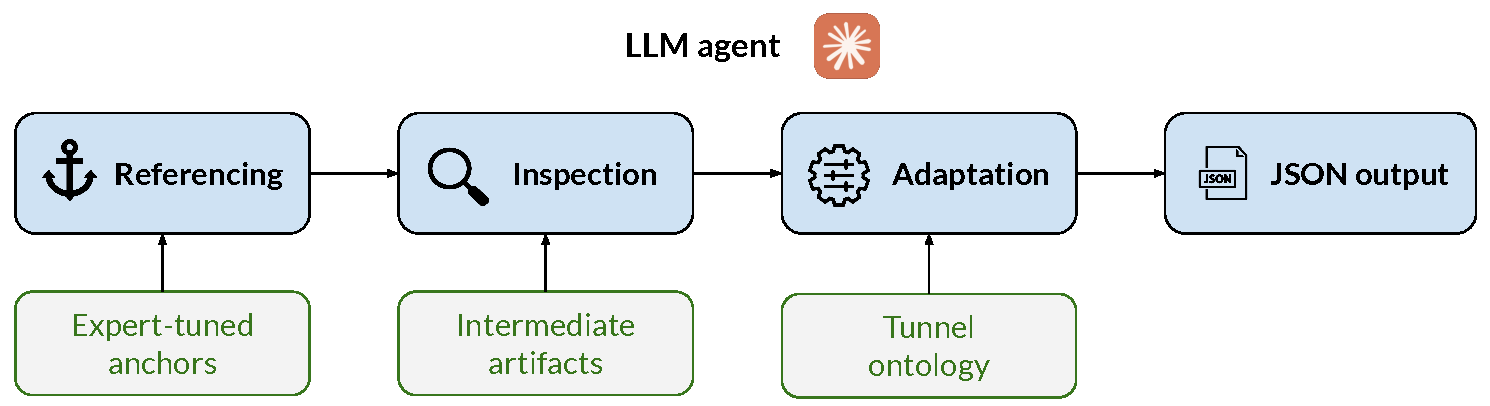
\includegraphics[width=0.8\textwidth]{figs/agent.pdf}
\caption{LLM-guided parameter proposals. The agent compares the current run with the family reference, inspects intermediate outputs and PQ/SC measurements, and returns a bounded parameter overlay with a rationale. After execution, the frozen proxy scores the candidate. Candidate retention depends only on the proxy score and a GT-free stage-1 tie-break.}
\label{fig:agent}
\end{figure*}

Each refinement attempt has three steps:
\begin{enumerate}
\item \textbf{Inspect and propose.}
The proposer returns one overlay. For the LLM arms this follows \emph{symptom} $\rightarrow$ \emph{evidence} $\rightarrow$ \emph{bounded parameter diff} $\rightarrow$ \emph{rationale}; for the random arm the overlay is drawn from the search space.
\item \textbf{Validate and execute.}
The overlay is checked against the family search space (parameter names, types, marginal bounds; stage-1 keys only when unlocked). A valid candidate is executed through stages~1--5 and its measurements are computed.
\item \textbf{Score and record.}
The frozen proxy estimates candidate accuracy. The base configuration, overlay, execution status, measurements, score, and stage-1 residual are recorded for subsequent feedback and final selection.
\end{enumerate}
Each admitted case receives three attempts without early stopping. Invalid or failed attempts are recorded, consume an attempt, and are excluded from selection.

\paragraph{Admission.}
The proxy score of the starting run is used once, before the loop, through the study operating bands
\begin{equation}
\operatorname{QC}(\hat y)=
\begin{cases}
\text{flag}, & \hat y<0.5,\\
\text{refine}, & 0.5\le\hat y<0.7,\\
\text{accept}, & \hat y\ge0.7,
\end{cases}
\label{eq:qc-bands}
\end{equation}
which illustrate assessment decisions and are not validated engineering acceptance criteria. Only ``refine'' starts enter the loop. The same band is applied to the retained output afterwards; a result may remain in the refine band after the fixed budget is exhausted.

\paragraph{Selection.}
Selection is monotone in the proxy and keeps the start eligible. Let $r=0$ be the start, $\mathcal V$ the scored candidates, $\hat y_r$ the clipped score, and $\eta_r$ the stage-1 recentring residual (cm). With $\mathcal C=\{r\in\mathcal V:\hat y_r>\hat y_0\}$ and $\mathcal C_\varepsilon=\{r\in\mathcal C:\hat y_r\ge\max_{\mathcal C}\hat y-\varepsilon\}$, $\varepsilon=0.01$,
\begin{equation}
r^\star=
\begin{cases}
0, & \mathcal C=\emptyset,\\
\operatorname*{arg\,min}_{r\in\mathcal C_\varepsilon}(\eta_r,\,-\hat y_r), & \text{otherwise},
\end{cases}
\label{eq:refinement-selection}
\end{equation}
where the minimisation is lexicographic: among near-tied candidates the lower residual, then the higher score, is preferred. The residual is a GT-free stage-1 quantity used only as a tie-break; Section~\ref{sec:poc-verification} also reports pure maximum-proxy selection to show how much it mattered. SC measurements contribute to the proxy and inform the agent's diagnosis but impose no separate retention gate. Algorithm~\ref{alg:reflective_adaptation} summarises the procedure.

\begin{algorithm}[!htb]
\caption{Proxy-guided parameter refinement}
\label{alg:reflective_adaptation}
\small
\begin{algorithmic}[1]
\Require Subset $D$; start $P_0$ (expert family reference); frozen proxy $g$; bounds; budget $R=3$; $\varepsilon=0.01$
\Ensure Retained configuration $P^\star$ and QC status
\State Execute $P_0$; if it fails or any measurement is non-finite, \Return $P_0$, flag
\State $\hat y_0\gets\operatorname{clip}(g(\mathbf x_0),0,1)$; $\eta_0\gets$ stage-1 residual
\If{$\hat y_0<0.5$ \textbf{or} $\hat y_0\ge0.7$} \Return $P_0$, $\operatorname{QC}(\hat y_0)$ \Comment{pre-loop return, Eq.~\eqref{eq:qc-bands}}
\EndIf
\State $\mathcal V\gets\emptyset$
\For{$r=1,\ldots,R$}
  \State Obtain overlay from the proposer (context: settings, outputs, measurements, scores, history)
  \State Validate overlay against bounds and stage-1 lock; \textbf{if} invalid, record and \textbf{continue}
  \State $P_r\gets\operatorname{Apply}(P_0,\text{overlay})$; run stages 1--5; \textbf{if} failure, record and \textbf{continue}
  \State $\hat y_r\gets\operatorname{clip}(g(\mathbf x_r),0,1)$; $\eta_r\gets$ residual; $\mathcal V\gets\mathcal V\cup\{r\}$
\EndFor
\State $r^\star\gets$ Eq.~\eqref{eq:refinement-selection}; $P^\star\gets P_{r^\star}$
\State \Return $P^\star$, $\operatorname{QC}(\hat y_{r^\star})$
\end{algorithmic}
\end{algorithm}

\paragraph{Information boundary.}
The scorer reads only the four measurements of the run being scored; the selector reads only proxy scores and residuals; and no GT label, GT value, or evaluation file of the scan under refinement is placed in any proposal prompt. One qualification remains: stage~1 uses the ring-index annotation as described in Section~\ref{sec:pipeline}. All three LLM arms use fresh per-case contexts resumed only for rounds 2--3 of the same case.

\subsection{Experimental design}
\label{sec:exp-setup}

The evaluation addresses three questions: whether PQ and SC support accuracy estimation that transfers across lining families, whether the frozen proxy distinguishes reference outputs from controlled degradations on unseen scans, and whether proxy-based selection produces useful parameter refinement, and if so, how much of that effect is attributable to the proposer.

\subsubsection{Dataset and use of annotations}
\label{sec:dataset}

We use Seg2Tunnel subsets from three lining families~\cite{lin2024seg2tunnel} (Table~\ref{tab:dataset}). Subsets 2-1, 3-1, and 5-1 are the development subsets and supply the 120 calibration records. The evaluation panel comprises 27 other subsets, nine per family, all excluded from proxy fitting. These subsets come from the represented families and tunnel collection, so the evaluation examines transfer to unseen scans within this setting rather than unrestricted transfer to new projects or lining geometries.

``Held out'' refers to proxy calibration only. The expert reference configurations for 1-1 and 4-1 were tuned on those scans' own GT and then reapplied to them, whereas the other 25 subsets receive reference settings established on a different scan of the same tunnel. Every stage-1 execution reads the ring-index annotation for frame orientation. The degraded overlays for the continuous and complex families were identified by GT from earlier exploration trials on evaluation subsets 3-2 and 4-1 (Section~\ref{sec:stress-test}). Evaluation labels are otherwise used only to measure performance and to define retrospective GT strata.

\begin{table*}[t]
\caption{Development and evaluation subsets, and every use of annotation-derived information. One labelled development subset per family supplies the calibration trials; nine other subsets per family form the evaluation panel, all excluded from proxy fitting.}
\label{tab:dataset}
\centering
\small
\setlength{\tabcolsep}{4pt}
\begin{tabular}{Y{0.20\textwidth} Y{0.22\textwidth} Y{0.22\textwidth} Y{0.26\textwidth}}
\toprule
Property & Staggered (T1, T2) & Continuous (T3) & Complex (T4, T5) \\
\midrule
Inner diameter / ring length & 5.5\,m / 1.2\,m & 5.9\,m / 1.2\,m & 7.5\,m / 1.8\,m \\
Blocks per ring; key layout & 6; ring-to-ring repeating & 6; fixed ring-wise order & 7; no repeating pattern \\
Scanning & Single-station & Multi-station & Single-station, offset \\
Development subset (40 runs) & 2-1 & 3-1 & 5-1 \\
Evaluation subsets & 1-1--1-5; 2-2--2-5 & 3-2--3-10 & 4-1--4-5; 5-2--5-5 \\
Reference source per tunnel & 1-1 (own GT); 2-1 & 3-1 profile & 4-1 (own GT); 5-1 \\
Degraded-overlay source (GT mIoU) & 2-1 trial (0.032) & 3-2 trial (0.027) & 4-1 trial (0.036) \\
\midrule
\multicolumn{4}{p{0.94\textwidth}}{Additional uses: every stage-1 run reads the ring-index annotation for frame orientation and validation.} \\
\bottomrule
\end{tabular}
\end{table*}

\subsubsection{Feature and model comparisons}
\label{sec:comparators}

The comparisons in Table~\ref{tab:proxy-ablation} use the same calibration trials and segmentation pipeline. We report training fit and LOFO performance separately. LOFO comparisons inform model development; evaluation on the 27 unseen subsets then tests the frozen proxy. The permutation control (Section~\ref{sec:ridge-proxy}) examines whether the measurements carry information about accuracy beyond differences between families; it does not itself establish the absence of leakage, which is enforced separately by GT isolation and fold-specific fitting.

\subsubsection{Paired degradation test}
\label{sec:stress-test}

Each evaluation subset is processed with its unmodified reference configuration and with a degraded counterpart, giving 27 pairs and 54 runs. The degradation rule was fixed before the proxy was frozen: for each family, the lowest-mIoU completed trial in an earlier parameter-exploration archive supplies a stage-2--5 overlay (Appendix~\ref{app:anchor-parameter}), applied unchanged on top of every subset's reference; stage-1 settings are inherited so that both members share a frame, and the full pipeline is rerun. No label or boundary is edited directly. All 54 runs executed and were scorable.

Both outputs in each pair are assessed with the same frozen feature definitions and proxy, and GT mIoU is calculated separately. The test examines whether the proxy ranks the reference above its degraded counterpart and whether the fixed low-quality threshold detects the constructed degradation. Because one overlay per family is reused on nine scans, the degraded runs represent three severe parameter failure modes (GT mIoU 0.03--0.12), not 27 independent or marginal failures; the panel supports conclusions about discrimination under these perturbations rather than operational false-alarm rates.

\subsubsection{Refinement panel and proposal arms}
\label{sec:poc-protocol}

The starting run of every evaluation subset is its reference run, shared with the degradation test. The 22 starts with $0.5\le\hat y_0<0.7$ form the refinement panel; three starts fall below and two above the band, and GT plays no part in admission. Each case receives three proposals from each of three LLM proposal systems, Fable~5.1, GPT-5.6, and Gemini~3.8, and from a fourth \emph{random-overlay} control arm, under an identical proxy, validator, budget, execution code, and selector (Fig.~\ref{fig:verification}; Appendix~\ref{app:panel-config}). All $264$ proposals ($22\times3\times4$) executed. Stage~1 was unlocked in four cases (3-4, 3-8, 3-10, 4-3).

The LLM arms are \emph{session-attributed proposal systems}, not verified model interventions. Model identifiers come from agent-interface sessions, not provider API records, and decoding settings were not controllable. Fable~5.1, GPT-5.6, and Gemini~3.8 each used a fresh per-case context resumed only for rounds 2--3 of that case; for Gemini~3.8 most cases had all three proposals prepared before execution. The LLM comparison is therefore exploratory and compares realised proposal systems, not intrinsic LLM capability.

The random-overlay arm asks whether an LLM is needed at all as the proposer. For each case it draws three overlays non-adaptively (all three before any execution) with a fixed seed. The number of changed parameters $k$ is sampled from the pooled empirical distribution of parameters that the three LLM arms actually changed relative to the reference on the 198 panel records (excluding $k=0$); the chosen parameters then receive values drawn uniformly within the family search-space bounds, with the same integer, Boolean, and radial-gate repairs as the calibration sampler, and with unfolding parameters available only when stage~1 is unlocked. Values are not step-size matched to the LLMs; the control matches proposal sparsity, not proposal geometry.

To separate the selector from the proposals, each arm is also summarised under reference policies applied to the same executed candidates: retain the start; always take round~1; a uniformly random round (reported as its expectation, the mean of the three rounds); pure maximum-proxy selection with the start eligible and no tie-break; and a GT oracle (best of start and three rounds). These are post-hoc fixed-pool comparisons; an adaptive proposer might have generated different later proposals under a different rule.

\begin{figure*}[t]
\centering
\resizebox{\textwidth}{!}{%
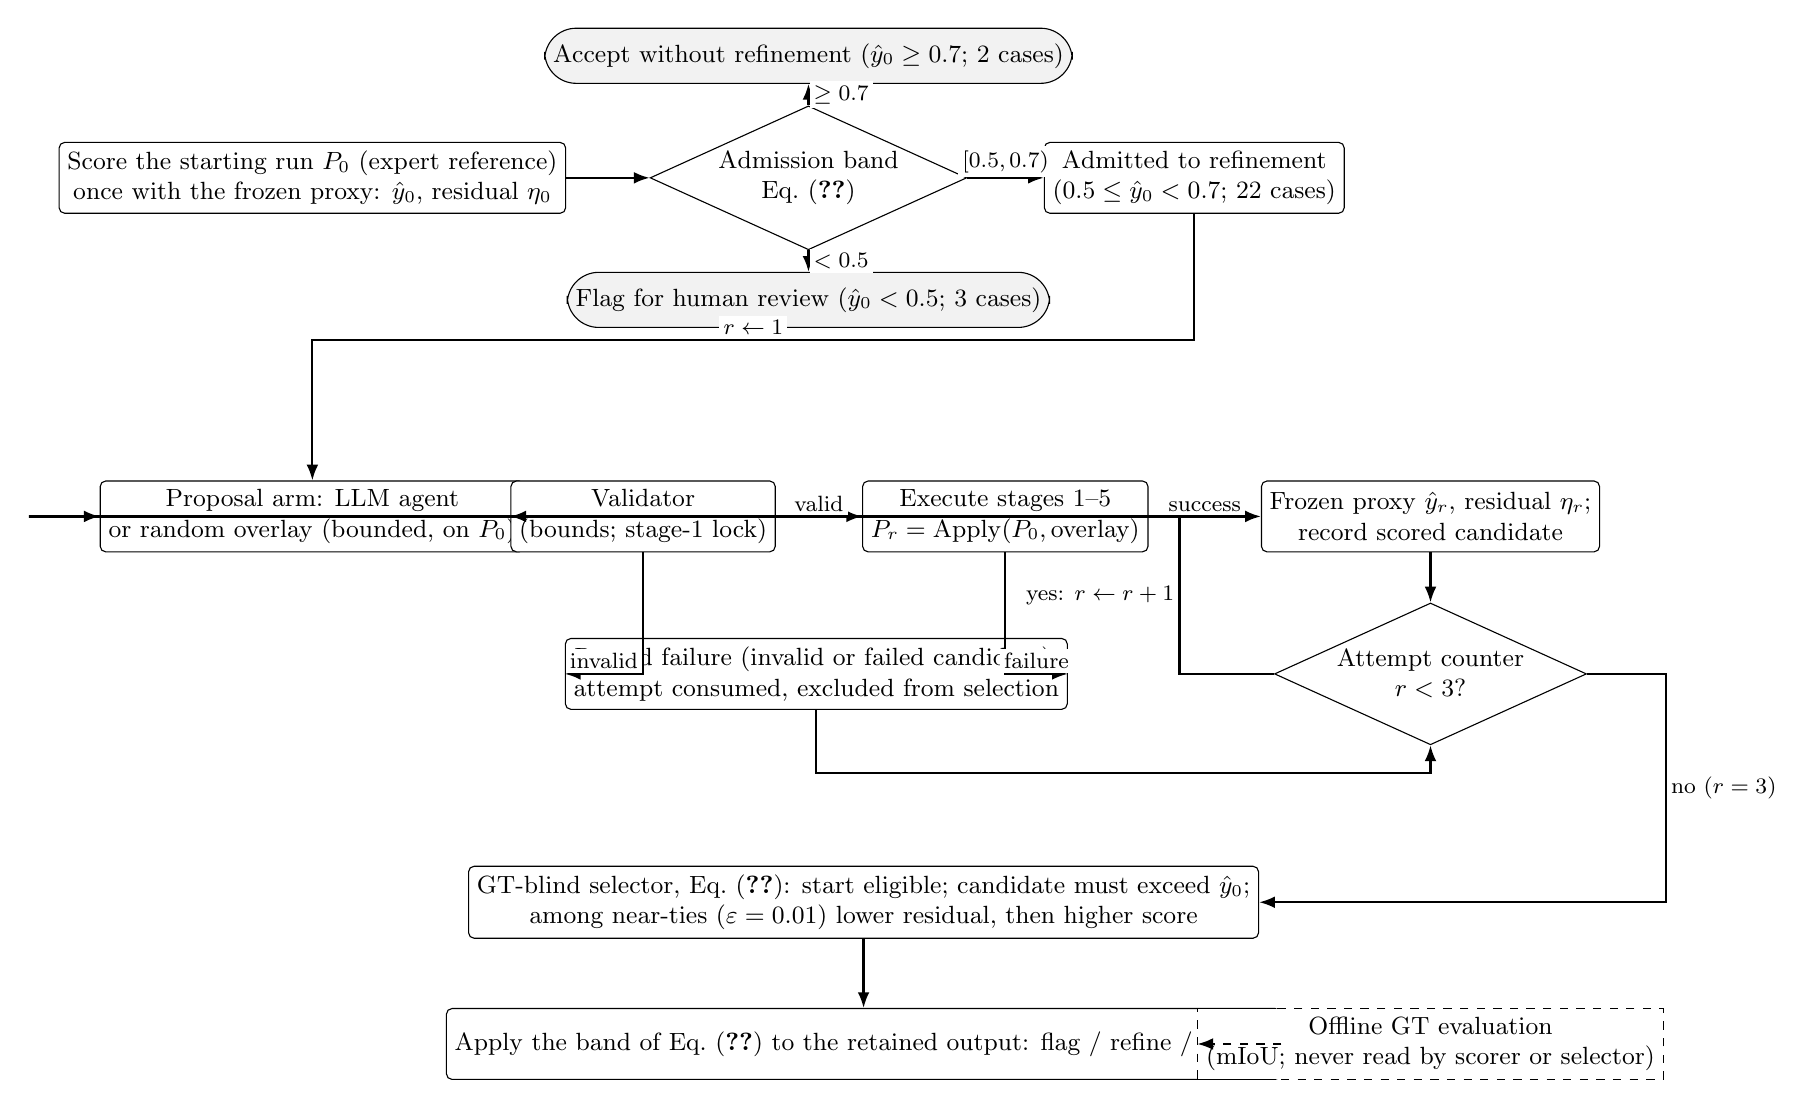
\begin{tikzpicture}[x=1cm,y=1cm,
  font=\small,
  box/.style={draw,rounded corners=2pt,align=center,minimum height=9mm,inner sep=3pt,fill=white},
  dec/.style={draw,diamond,aspect=2.2,align=center,inner sep=1pt,fill=white},
  term/.style={draw,rounded corners=4mm,align=center,minimum height=7mm,inner sep=3pt,fill=gray!10},
  gt/.style={draw,dashed,align=center,minimum height=8mm,inner sep=3pt,fill=white},
  arr/.style={-{Latex[length=2mm]},thick},
  lab/.style={font=\footnotesize,fill=white,inner sep=1.5pt}]
% ---------- Row 1: single admission decision ----------
\node[box] (score0) at (0,0) {Score the starting run $P_0$ (expert reference)\\once with the frozen proxy: $\hat y_0$, residual $\eta_0$};
\node[dec] (adm) at (6.3,0) {Admission band\\Eq.~\eqref{eq:qc-bands}};
\node[box] (admit) at (11.2,0) {Admitted to refinement\\($0.5\le\hat y_0<0.7$; 22 cases)};
\node[term] (acc0) at (6.3,1.55) {Accept without refinement ($\hat y_0\ge0.7$; 2 cases)};
\node[term] (flag0) at (6.3,-1.55) {Flag for human review ($\hat y_0<0.5$; 3 cases)};
\draw[arr] (score0) -- (adm);
\draw[arr] (adm.east) -- node[lab,above]{$[0.5,0.7)$} (admit.west);
\draw[arr] (adm.north) -- node[lab,right]{$\ge0.7$} (acc0.south);
\draw[arr] (adm.south) -- node[lab,right]{$<0.5$} (flag0.north);
% ---------- Row 2: fixed-budget loop ----------
\node[box] (prop) at (0,-4.3) {Proposal arm: LLM agent\\or random overlay (bounded, on $P_0$)};
\node[box] (val) at (4.2,-4.3) {Validator\\(bounds; stage-1 lock)};
\node[box] (exec) at (8.8,-4.3) {Execute stages 1--5\\$P_r=\operatorname{Apply}(P_0,\text{overlay})$};
\node[box] (scorer) at (14.2,-4.3) {Frozen proxy $\hat y_r$, residual $\eta_r$;\\record scored candidate};
\node[box] (fail) at (6.4,-6.3) {Record failure (invalid or failed candidate);\\attempt consumed, excluded from selection};
\node[dec] (cnt) at (14.2,-6.3) {Attempt counter\\$r<3$?};
\draw[arr] (admit.south) |- ($(admit.south)+(0,-1.6)$) -| node[lab,pos=0.25,above]{$r\gets1$} (prop.north);
\draw[arr] (prop) -- (val);
\draw[arr] (val) -- node[lab,above]{valid} (exec);
\draw[arr] (exec) -- node[lab,above]{success} (scorer);
\draw[arr] (val.south) |- node[lab,pos=0.75,above]{invalid} (fail.west);
\draw[arr] (exec.south) |- node[lab,pos=0.75,above]{failure} (fail.east);
\draw[arr] (scorer.south) -- (cnt.north);
\draw[arr] (fail.south) |- ($(fail.south)+(0,-0.8)$) -| (cnt.south);
\draw[arr] (cnt.west) -- ++(-1.2,0) |- node[lab,pos=0.25,left]{yes: $r\gets r+1$} ($(prop.west)+(-0.9,0)$) -- (prop.west);
% ---------- Row 3: selection ----------
\node[box] (sel) at (7.0,-9.2) {GT-blind selector, Eq.~\eqref{eq:refinement-selection}: start eligible; candidate must exceed $\hat y_0$;\\among near-ties ($\varepsilon=0.01$) lower residual, then higher score};
\node[box] (band) at (7.0,-11.0) {Apply the band of Eq.~\eqref{eq:qc-bands} to the retained output: flag / refine / accept};
\node[gt] (gtb) at (14.2,-11.0) {Offline GT evaluation\\(mIoU; never read by scorer or selector)};
\draw[arr] (cnt.east) -- ++(1.0,0) |- node[lab,pos=0.25,right]{no ($r=3$)} ($(sel.east)+(0.5,0)$) -- (sel.east);
\draw[arr] (sel) -- (band);
\draw[arr,dashed] (band.east) -- (gtb.west);
\end{tikzpicture}}
\caption{Refinement protocol. Top: the frozen proxy scores the starting run once and the band admits, accepts, or flags it. Middle: each of three attempts yields one bounded overlay from the proposal arm (an LLM agent or the random-overlay control) that is validated, executed, and scored; failures consume an attempt. Bottom: the GT-blind selector chooses among the start and scored candidates, and the band is applied to the retained output. GT is read only by the offline evaluator.}
\label{fig:verification}
\end{figure*}

\subsubsection{Evaluation metrics and uncertainty}
\label{sec:metrics}

Offline segmentation accuracy is point-level semantic mIoU over the whole subset with labels background plus the positional block classes ($C=7$ for staggered and continuous, $8$ for complex). With $\mathcal A=\{c:\operatorname{TP}_c+\operatorname{FP}_c+\operatorname{FN}_c>0\}$ the set of classes present in GT or prediction,
\begin{equation}
\operatorname{IoU}_c
=
\frac{\operatorname{TP}_c}
{\operatorname{TP}_c+\operatorname{FP}_c+\operatorname{FN}_c},
\qquad
\operatorname{mIoU}
=
\frac{1}{|\mathcal A|}\sum_{c\in\mathcal A}\operatorname{IoU}_c ,
\end{equation}
where IoU is pooled over points per class and background is included whenever it belongs to $\mathcal A$. Points removed by denoising or outside every SAM mask count as background, so lost lining points are false negatives. In every reported subset all $C$ classes occur in GT, so $|\mathcal A|=C$ throughout.

Proxy fidelity is reported as mean absolute error
\begin{equation}
\operatorname{MAE}
=
\frac{1}{n}\sum_{i=1}^{n}
|\hat{y}_i-y_i|
\end{equation}
against GT mIoU, and Spearman $\rho$, which measures whether the proxy orders runs consistently with GT accuracy. For the paired degradation test, ranking accuracy is
\begin{equation}
\operatorname{PairRank}
=
\frac{1}{M}\sum_{s=1}^{M}
\mathbb{I}
\left[
\hat{y}_{s,\mathrm{ref}}>
\hat{y}_{s,\mathrm{deg}}
\right],
\end{equation}
where $M=27$ and tied scores do not count as successful rankings. Alarm precision and recall are calculated at the fixed threshold of 0.5 against the reference/degraded construction labels. The primary interval for $\rho$ is a percentile bootstrap that resamples \emph{subsets} within family (pairs kept together; 2000 replicates, seed 0). Because subsets of one parent tunnel are dependent, a sensitivity interval enumerates all $5^5$ ordered resamples of the five parent tunnels.

For refinement, the case effect $\Delta_i$ is the GT mIoU of the selected output minus that of the start. We report mean and median $\Delta$, improved/unchanged/harmed counts at three-decimal precision, worst harm, family and GT-stratum means, and 95\% intervals from a paired parent-tunnel cluster bootstrap (five clusters; 100{,}000 resamples; fixed seed). With five clusters these intervals are coarse, and with one realised trajectory per case and arm they exclude proposer stochasticity. Efficiency is described by proposal yield (candidates whose proxy exceeds the start), accepted-proposal precision (of those, the fraction whose GT mIoU also exceeds the start), selector regret (best available GT mIoU minus selected GT mIoU), and segmentation compute; LLM latency and cost are not compared because commensurate metadata are unavailable.

% ═════════════════════════════════════════════════════════════════════════
\section{Results}\label{sec:results}

The results follow the three questions of Section~\ref{sec:exp-setup}: Section~\ref{sec:main-results} compares feature sets on the calibration runs; Section~\ref{sec:degradation-results} tests the frozen proxy on the 54 stress-test runs; Sections~\ref{sec:poc-verification}--\ref{sec:efficiency-results} report the four-arm refinement panel and separate the selector from the proposers; and Section~\ref{sec:error-analysis} analyses where the proxy, the segmentation, and the selector err.

\subsection{Proxy calibration and transfer between families}\label{sec:main-results}

Table~\ref{tab:ablation-results} and Fig.~\ref{fig:ablation_results}a compare feature sets on the 120 development runs. The ten-feature model fits the calibration data most closely but transfers worst among the combined models; the four-feature compact model has the highest LOFO correlation (0.828) and lowest LOFO MAE (0.112). Across the eight nested candidates LOFO $\rho$ ranged from 0.723 (six features) to 0.828 (four); dropping the missing-depth rate to three features gave 0.794. SC alone transfers better than PQ alone, while the compact combination of one PQ and three SC measurements transfers better than either group on its own. The folds differ substantially: held-out continuous $\rho=0.627$ against 0.942 (staggered) and 0.915 (complex), so transfer to the multi-station continuous family is the weakest link in the calibration evidence. Within-family label permutation raises MAE to $0.196\pm0.008$ and lowers $\rho$ to $0.202\pm0.089$ (20 repeats), so the association is not an artefact of family means. These figures condition on parameter variation around three scans and, having been used to choose the feature set, are diagnostics rather than unbiased transfer estimates.

\begin{table*}[t]
\caption{Feature-set comparison on the 120 development runs. LOFO: leave-one-family-out, mean of three folds. Per-fold LOFO for the deployed model: staggered $\rho=0.942$, MAE 0.122; continuous 0.627, 0.125; complex 0.915, 0.088. Permutation control (deployed set, 20 within-family shuffles): $\rho=0.202\pm0.089$, MAE $0.196\pm0.008$.}\label{tab:ablation-results}
\centering
\begin{tabular*}{\textwidth}{@{\extracolsep{\fill}} l c cc cc @{}}
\toprule
& & \multicolumn{2}{c}{Training fit} & \multicolumn{2}{c}{LOFO} \\
\cmidrule(lr){3-4} \cmidrule(lr){5-6}
Feature set & \#Features & $\rho$ & MAE & $\rho$ & MAE \\
\midrule
PQ only, $P(q)$ & 4 & 0.785 & 0.108 & 0.597 & 0.155 \\
SC only, $P(c)$ & 6 & 0.897 & 0.086 & 0.766 & 0.139 \\
Combined, $P(q{+}c)$ & 10 & 0.915 & 0.081 & 0.794 & 0.197 \\
Compact $P(q{+}c)$ (deployed) & \textbf{4} & 0.904 & 0.086 & \textbf{0.828} & \textbf{0.112} \\
\bottomrule
\end{tabular*}
\end{table*}

The selected proxy contains one PQ and three SC measurements: missing-depth rate, correspondence F1@15, fill rate, and ring-count residual. With standardised inputs $z_j$, the frozen proxy is
\begin{equation}
\begin{aligned}
\hat y={}&0.350+0.0823z_{\mathrm{corr}}+0.0798z_{\mathrm{fill}}\\
&-0.0454z_{\mathrm{ringerr}}-0.0644z_{\mathrm{nan}},
\end{aligned}
\label{eq:lean-proxy}
\end{equation}
with $\alpha=10$ and constants in Appendix~\ref{app:proxy-package}. Positive correspondence and fill coefficients associate higher scores with segmentations that are populated and supported by detected joint evidence; negative ring-count and missing-depth coefficients associate lower scores with implausible ring counts and incomplete depth maps. These are conditional associations in a correlated linear model, not independent causal effects or instructions for changing parameters.

\begin{figure*}[t]
\centering

\includegraphics[width=\textwidth]{figs/ablation_results.pdf}
\caption{Proxy calibration and frozen evaluation. (a)~On the 120 calibration trials (40 per development subset), the compact four-feature model preserves training fit close to the ten-feature model while transferring better between families (Table~\ref{tab:ablation-results}); trend lines show the fitted association of each feature set. (b)~The frozen proxy is then evaluated, without refitting, on 54 runs from 27 held-out subsets: 27 reference runs (circles) and their 27 degraded counterparts (crosses). The dashed line is the alarm threshold $\hat y<0.5$; the shaded band $[0.5,0.7)$ is the refine band from which the 22 refinement cases are admitted. GT is used only on the horizontal axis.}
\label{fig:ablation_results}
\end{figure*}

\subsection{Paired degradation test}\label{sec:degradation-results}

On the 54 evaluation runs the frozen proxy reaches $\rho=0.817$ and MAE 0.109 (Table~\ref{tab:holdout-fidelity}; Fig.~\ref{fig:ablation_results}b). It ranks the reference above its degraded counterpart in all 27 pairs and, at the 0.5 threshold, flags all 27 degraded runs and three reference runs (3-2, 3-5, and 4-4, whose GT mIoU is 0.631, 0.588, and 0.347). The two interval constructions agree on the direction of the result but differ in width: resampling subsets gives $[0.761,0.864]$, resampling parent tunnels $[0.718,0.921]$, so the dependence structure matters at the second decimal.

\begin{table}[ht]
\caption{Frozen-proxy fidelity on the 54 stress-test runs (27 reference, 27 degraded). Intervals: subset bootstrap within family (primary) and enumeration of all $5^5$ parent-tunnel resamples (sensitivity).}
\label{tab:holdout-fidelity}
\setlength{\tabcolsep}{4pt}
\begin{tabular*}{\tblwidth}{@{\extracolsep{\fill}} l c @{}}
\toprule
Metric & Value \\
\midrule
Spearman $\rho$ & 0.817 \\
\quad subset-bootstrap 95\% CI & [0.761, 0.864] \\
\quad parent-cluster interval & [0.718, 0.921] \\
MAE overall & 0.109 \\
MAE stag.\ / cont.\ / compl. & 0.126 / 0.122 / 0.078 \\
Pairs ranked correctly & 27/27 \\
Alarms ($\hat y<0.5$), degraded; reference & 27/27; 3/27 \\
Alarm precision / recall & 0.90 / 1.00 \\
\bottomrule
\end{tabular*}
\end{table}

Ranking and numerical fidelity diverge. An MAE of 0.109 is about half the width of the 0.2-wide refine band, and the proxy under-estimates accurate outputs: the 22 admitted starts have mean proxy 0.606 against mean GT mIoU 0.738, which is why 16 of the 22 ``refine'' cases were already above 0.7 GT mIoU. Perfect pairwise ranking of severe degradations therefore coexists with absolute estimates too coarse for acceptance decisions.

\subsection{Proxy-guided refinement with four proposal arms}\label{sec:poc-verification}

From a common start, selected mean mIoU rises to 0.751 (Fable~5.1), 0.760 (GPT-5.6), 0.759 (Gemini~3.8), and 0.752 (random); every pairwise cluster-bootstrap interval among the four arms includes zero (Table~\ref{tab:panel-miou}; Fig.~\ref{fig:refinement_results}a). Median gains are 0.000: the means are driven by a few large improvements. Ranking by mean is not ranking by safety---worst case losses span $-0.195$ (Fable~5.1) to $-0.117$ (random).

\begin{table*}[t]
\caption{Paired refinement results on the 22-case proxy-admitted panel. 95\% CIs: parent-tunnel cluster bootstrap. Up/same/down at three-decimal precision. Pairwise mean differences: Fable$-$GPT $-0.009$ $[-0.033,+0.025]$; Fable$-$Gemini $-0.008$ $[-0.033,+0.019]$; Fable$-$random $-0.001$ $[-0.038,+0.043]$; GPT$-$Gemini $+0.001$ $[-0.049,+0.048]$; GPT$-$random $+0.008$ $[-0.010,+0.022]$; Gemini$-$random $+0.007$ $[-0.049,+0.066]$.}\label{tab:panel-miou}
\centering
\small
\setlength{\tabcolsep}{3pt}
\begin{tabular*}{\textwidth}{@{\extracolsep{\fill}} l c c c c c c c c}
\toprule
Arm & Proxy & mIoU & Mean $\Delta$ & Median $\Delta$ & 95\% CI & Refined & Up / same / down & Worst $\Delta$ \\
\midrule
Start (common) & 0.606 & 0.738 & -- & -- & -- & -- & -- & -- \\
Fable~5.1 & 0.631 & 0.751 & $+0.013$ & 0.000 & $[-0.017,+0.052]$ & 21/22 & 9 / 4 / 9 & $-0.195$ \\
GPT-5.6 & 0.629 & 0.760 & $+0.022$ & 0.000 & $[-0.014,+0.077]$ & 15/22 & 7 / 7 / 8 & $-0.091$ \\
Gemini~3.8 & 0.641 & 0.759 & $+0.021$ & $+0.003$ & $[+0.009,+0.044]$ & 18/22 & 12 / 7 / 3 & $-0.024$ \\
Random & 0.628 & 0.752 & $+0.014$ & 0.000 & $[-0.028,+0.078]$ & 16/22 & 8 / 8 / 6 & $-0.117$ \\
\bottomrule
\end{tabular*}
\end{table*}

Table~\ref{tab:selector-policies} and Fig.~\ref{fig:refinement_results}b isolate the selector on the same candidates. Unselected proposals harm three of four arms on average; the monotone-accept selector recovers 47--78\% of the GT-oracle gain. Max-proxy matches monotone-accept for almost every case--arm pair (one Gemini~3.8 tie-break on 3-4). The collapse and recovery of unselected random proposals is the strongest within-study evidence that proxy ranking with the start eligible, not proposer identity, carries the gain.

\begin{table*}[t]
\caption{Mean mIoU on the 22-case panel under alternative selection policies applied to the same executed candidates. All policies except the oracle are GT-blind and deployable; all are evaluated with GT. Random round is reported as its expectation (mean of three rounds). Oracle recovery $=$ (monotone-accept $-$ start)/(oracle $-$ start). Post-hoc fixed-pool comparison.}\label{tab:selector-policies}
\centering
\small
\begin{tabular*}{\textwidth}{@{\extracolsep{\fill}} l c c c c c c c}
\toprule
Arm & Start & Random round & Round~1 & Max-proxy & Monotone-accept & GT oracle & Oracle recovery \\
\midrule
Fable~5.1 & 0.738 & 0.734 & 0.714 & 0.751 & 0.751 & 0.765 & 49\% \\
GPT-5.6 & 0.738 & 0.706 & 0.683 & 0.760 & 0.760 & 0.770 & 69\% \\
Gemini~3.8 & 0.738 & 0.715 & 0.692 & 0.757 & 0.759 & 0.765 & 78\% \\
Random & 0.738 & 0.535 & 0.508 & 0.752 & 0.752 & 0.769 & 47\% \\
\bottomrule
\end{tabular*}
\end{table*}

\begin{figure*}[t]
\centering

\includegraphics[width=\textwidth]{figs/refinement_results.pdf}
\caption{Proxy-guided refinement on the 22 proxy-admitted cases. (a)~Mean GT mIoU of the selected output by proposal arm; error bars are 95\% parent-tunnel cluster-bootstrap intervals on the paired gain, drawn around the arm mean. (b)~The same executed candidates under four selection policies (Table~\ref{tab:selector-policies}): unselected proposals (random round, round~1) fall below the start for three of four arms, whereas the shared GT-blind proxy selector recovers 47--78\% of the GT-oracle gain. (c)~Per-case gain against starting GT mIoU for all four arms: gains concentrate on the six starts below 0.7 GT mIoU; the remaining 16 cases change little in either direction.}
\label{fig:refinement_results}
\end{figure*}

\subsection{Where the gains occur}\label{sec:regional-results}

Gains concentrate on staggered tunnels and on the six starts with GT mIoU below 0.7; continuous and already-accurate cases barely move (Table~\ref{tab:gt-strata}; Fig.~\ref{fig:refinement_results}c). Subset 1-5 alone can supply about half of an LLM arm's positive gain. Excluding the two self-tuned references (1-1, 4-1) leaves the panel means essentially unchanged. The complete case table is Appendix~\ref{app:poc-selection}. These GT strata are retrospective and cannot serve as a deployment rule.

\begin{table*}[t]
\caption{Mean $\Delta$mIoU by lining family and by starting GT mIoU (retrospective strata for all arms).}\label{tab:gt-strata}
\centering
\begin{tabular*}{\textwidth}{@{\extracolsep{\fill}} l c rrrr}
\toprule
Group & $n$ & Fable~5.1 & GPT-5.6 & Gemini~3.8 & Random \\
\midrule
Staggered & 7 & $+0.068$ & $+0.076$ & $+0.045$ & $+0.065$ \\
Continuous & 7 & $-0.005$ & $+0.001$ & $+0.011$ & $-0.026$ \\
Complex & 8 & $-0.019$ & $-0.007$ & $+0.009$ & $+0.005$ \\
\addlinespace
Start GT mIoU $<0.7$ & 6 & $+0.084$ & $+0.102$ & $+0.054$ & $+0.086$ \\
Start GT mIoU $\ge0.7$ & 16 & $-0.014$ & $-0.008$ & $+0.009$ & $-0.012$ \\
\bottomrule
\end{tabular*}
\end{table*}

\subsection{Proposal yield and compute}\label{sec:efficiency-results}

All 66 candidates per arm executed ($264$ in total). Fable~5.1 produced 43 proxy-improving candidates, of which 17 (39.5\%) also improved GT mIoU; GPT-5.6 produced 22, of which 12 (54.5\%); Gemini~3.8 produced 36, of which 18 (50.0\%); random produced 25, of which 14 (56.0\%). Mean selector regret was 0.014, 0.010, 0.006, and 0.017, respectively. Segmentation compute was similar across arms (mean 231--244\,s per run on one NVIDIA RTX~5060 GPU for the LLM arms; the random arm used the same execution path) and says nothing about LLM inference cost.

\subsection{Error analysis}\label{sec:error-analysis}

Three questions remain: where the proxy's numerical error comes from, which segmentation errors refinement removes, and why the selector sometimes retains a worse output. Point-level outcomes are classified against GT as \emph{correct}; \emph{false negative} (FN, a lining point predicted as background); \emph{false positive} (FP, a background point predicted as lining); and \emph{class swap} (a lining point assigned to the wrong lining block). Fractions are of all points in a subset (Table~\ref{tab:error-composition}; Fig.~\ref{fig:error_maps}).

\paragraph{Proxy error.}
On the 54 stress-test runs the signed error $\hat y-y$ is one-directional within each group: reference runs are under-estimated by 0.124 on average (staggered $-0.093$, continuous $-0.198$, complex $-0.081$) and degraded runs over-estimated by 0.076. The two directions together describe range compression, as expected from a regularised linear model whose predictions shrink towards the calibration mean. Two of the four measurements saturate on the degraded runs (missing-depth rate 0.89, fill rate 0.04 on average, against 0.16 and 0.71 for reference runs), and the ring-count residual is zero in all 54 runs, so the order \emph{within} the reference group rests on correspondence and, to a lesser extent, fill. Reference-run correspondence F1 averages 0.37, 0.24, and 0.30 by family, and the three reference alarms are the three reference runs with the lowest F1 (0.057, 0.124, and 0.071 for 3-2, 3-5, and 4-4): their correspondence contribution is negative ($-0.061$, $-0.024$, $-0.053$) while the other three terms are positive. Two of these are moderately accurate outputs (GT mIoU 0.631 and 0.588) on multi-station continuous scans with weak detected joint evidence; the third (4-4, GT mIoU 0.347) is a poor output that the construction labels count as a false alarm.

\begin{table}[ht]
\caption{Point-level error composition (\% of all points, mean over subsets). Degraded and reference: the 27 stress-test pairs. Start and arms: the 22 admitted cases, with the selected output of each arm. Refinement changes the swap fraction; FN and FP move by at most 0.3 points.}
\label{tab:error-composition}
\centering
\setlength{\tabcolsep}{4pt}
\begin{tabular*}{\tblwidth}{@{\extracolsep{\fill}} l r r r r @{}}
\toprule
Output & Correct & FN & FP & Swap \\
\midrule
Degraded (27) & 27.7 & 68.6 & 3.2 & 0.5 \\
Reference (27) & 84.2 & 3.6 & 5.2 & 7.1 \\
\addlinespace
Start (22) & 85.5 & 2.6 & 5.3 & 6.6 \\
Fable~5.1 selected & 86.3 & 2.7 & 5.3 & 5.7 \\
GPT-5.6 selected & 86.8 & 2.4 & 5.5 & 5.4 \\
Gemini~3.8 selected & 86.5 & 2.5 & 5.5 & 5.6 \\
Random selected & 86.3 & 2.7 & 5.5 & 5.4 \\
\bottomrule
\end{tabular*}
\end{table}

\paragraph{Segmentation error.}
The degraded overlays act by removing lining points: 68.6\% of all points become false negatives (Fig.~\ref{fig:error_maps}a), which is why the missing-depth and fill terms detect every one of them. Reference runs err differently: 7.1\% swaps, 5.2\% FP, 3.6\% FN. The error maps show that swaps occur as whole-ring bands (Fig.~\ref{fig:error_maps}b, d): when the key block of a ring is mislocated, the template labelling inherited from SAM4Tun rotates every block in that ring, the same mechanism identified for the unmodified pipeline in~\cite{taoR4Tun}. Refinement acts on this error type and on little else. Over the 22 cases the swap fraction falls from 6.6\% to 5.4--5.7\% depending on the arm, while FN and FP change by at most 0.3 points; the reduction is concentrated on the staggered family (8.9\% at the start; 4.7, 4.9, 6.6, and 5.5\% after Fable~5.1, GPT-5.6, Gemini~3.8, and random selection), where the gain in Table~\ref{tab:gt-strata} also concentrates. Continuous starts lose points instead (6.1\% FN, the largest of any family) and complex starts over-segment (8.3\% FP); neither fraction is reduced by any arm (5.2--7.0\% and 8.3--8.5\%), so the two families with little gain fail in ways that the permitted stage-2--5 changes did not repair within three attempts.

\begin{figure*}[t]
\centering
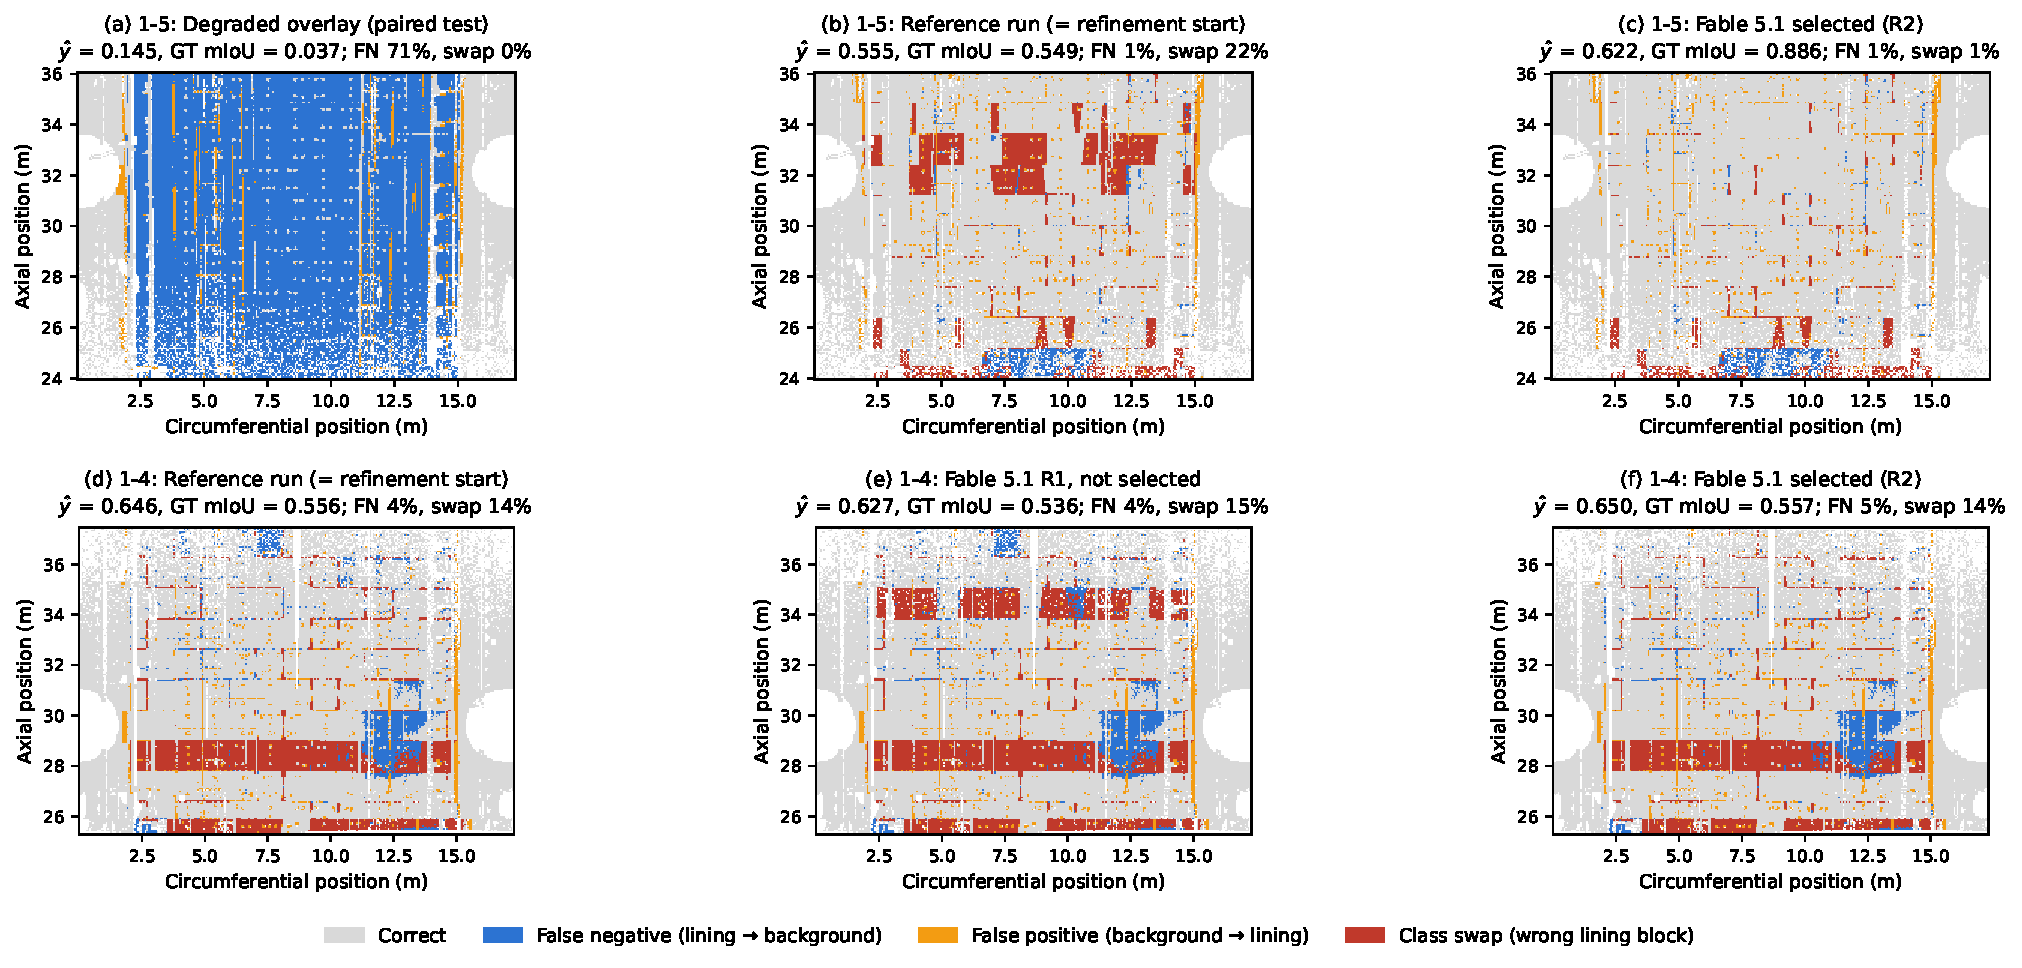
\includegraphics[width=\textwidth]{figs/error_maps.pdf}
\caption{Per-point error maps on the unfolded lining surface (horizontal: circumferential arc position; vertical: axial position; both in metres), classified against GT. Top row, subset 1-5: (a)~the degraded overlay of the paired test removes lining points (71\% FN) and scores $\hat y=0.145$; (b)~the reference run, which is also the refinement start, is dominated by whole-ring class swaps (22\%); (c)~the Fable~5.1 output retained by the selector (round~2, GT mIoU 0.886) removes most rotated rings (swap 2\%). Bottom row, subset 1-4: (d)~the start; (e)~round~1, GT mIoU 0.536, not selected; (f)~round~2, GT mIoU 0.557, selected because its proxy is higher. White regions are scan gaps; cells are coloured by an error type when it covers at least 30\% of their points.}
\label{fig:error_maps}
\end{figure*}

\paragraph{Selector error.}
Of 264 candidates, 118 scored above their start and 68 of these (57.6\%) also improved GT mIoU; of 146 rejected candidates, 17 (11.6\%) would have improved GT. Admission precision rises with $\Delta\hat y$ (23\% for $\le0.01$, 90\% above 0.05). Within a case the proxy moves almost only through correspondence. Fig.~\ref{fig:error_maps}e--f shows a near-flat case on 1-4 under Fable~5.1: rounds~1 and~2 score 0.627 and 0.650 while GT mIoU is 0.536 and 0.557---small proxy gains need not track useful accuracy change when joints stay fixed. A minimum admission margin and a label-order term are candidate remedies, neither evaluated here.

% ═════════════════════════════════════════════════════════════════════════
\section{Discussion}\label{sec:discussion}

What Proxy4Tun delivers is a frozen estimate that can compare bounded candidates of the same scan, and a retained-start selector that turns any such proposal pool into a modest mean gain. The qualifications that follow bound that claim; they do not reverse it.

The four measurements transfer better as a compact set than as PQ-only, SC-only, or the full ten-feature model, and on scans excluded from fitting they order every reference above its degraded counterpart. That supports \emph{comparison} of outputs of the same scan. Absolute acceptance is not supported: MAE 0.109, systematic under-estimation of accurate outputs, three reference alarms, and the severity of the constructed degradations limit what the 0.5/0.7 bands mean for engineering certification.

Unselected proposals lower the mean for three of four arms---catastrophically for random---while the shared GT-blind selector lifts all four arms and recovers most of the GT-oracle gain. The start is retained when nothing scores higher, so the proxy score is non-decreasing, not the accuracy: small proxy gains can still select whole-ring label rotations to which the four measurements are blind. The LLM arms differ mainly in risk profile; edges over this sparsity-matched random control are small and statistically unresolved. The study therefore does not establish that an LLM proposer is required once a retained-start proxy selector is in place.

Benefit concentrates on the few low-accuracy starts; the accurate majority barely moves, and a single staggered subset can supply about half of an arm's positive gain. The panel mean therefore overstates how widely benefit is distributed. An observable signal that separates an under-estimated accurate output from one that can still benefit is the natural next step.

\subsection{Comparison with existing paradigms}\label{sec:positioning}

Comparisons here concern operating points, not accuracy leaderboards (Table~\ref{tab:sota}). Supervised 3D models on Seg2Tunnel report strong in-distribution accuracy~\cite{lin2024seg2tunnel} but require per-point labels and GPU re-training for each new lining family, and provide no deployment-time accept/refine/flag gate. SAM4Tun reaches high accuracy on curated rings tuned case by case~\cite{ye2025sam4tun}, but a single fixed configuration transfers imperfectly off the reference scan (mean 0.722 over the 27 evaluation subsets here) and the pipeline emits no signal when it degrades. Relative to that static pipeline, Proxy4Tun adds an explicit accept/refine/flag gate without deployment labels. Relative to one-shot LLM parameter adapters such as R4Tun~\cite{taoR4Tun}, it adds a calibrated numeric proxy, so refinement can be \emph{assessed and selected} by an explicit estimated-quality signal rather than merely proposed; the random-control arm shows that this selection is where most of the benefit lies.

\begin{table*}[t]
\caption{Positioning Proxy4Tun against representative tunnel-segmentation paradigms by setup cost and deployment capability. \checkmark{} indicates the requirement (or capability) applies, ``--'' that it does not. \emph{Deep-learning training} refers to training or fine-tuning a segmentation network; Proxy4Tun fits only a separate linear proxy on offline labelled development data. mIoU figures are \emph{not} measured under comparable settings: supervised and expert-tuned figures are taken from~\cite{lin2024seg2tunnel} and~\cite{ye2025sam4tun} under their original protocols, whereas the Proxy4Tun figures are from this study on the 27 evaluation subsets: 0.722 for the fixed expert reference, and 0.732 after proxy-admitted refinement of 22 cases with the Fable~5.1 arm (0.739 for GPT-5.6 and Gemini~3.8; 0.733 for random), with the five non-admitted subsets unchanged.}\label{tab:sota}
\small
\begin{tabular*}{\textwidth}{@{\extracolsep{\fill}} Y{0.25\textwidth} c c c Y{0.24\textwidth} @{}}
\toprule
Method & \begin{tabular}[t]{@{}c@{}}Deep-learning\\training\end{tabular} & \begin{tabular}[t]{@{}c@{}}Per-case\\tuning\end{tabular} & \begin{tabular}[t]{@{}c@{}}Deployment-label-free\\quality signal\end{tabular} & mIoU (setting) \\
\midrule
LiningNet / SparseUNet / SCF-Net / FA-ResNet & \checkmark & -- & -- & 0.83--0.90 (supervised, in-distribution) \\
SAM4Tun & -- & Expert & -- & above 0.90 (per-case tuned rings) \\
SAM4Tun, fixed family reference & -- & -- & -- & 0.722 (27 evaluation subsets) \\
\textbf{Proxy4Tun} (compact $P(q{+}c)$) & -- & \textbf{Bounded, auto} & \checkmark & \textbf{0.732--0.739} (27 subsets, by arm) \\
\bottomrule
\end{tabular*}
\end{table*}

\subsection{Practical implications}

Each pipeline release needs one expert reference per lining family and one offline calibration. The frozen proxy then gives each new run a deployment-label-free mIoU estimate and an accept/refine/flag decision, and a retained-start selector turns any bounded proposer into a loop that filters harmful changes. The same calibration-and-selection pattern can extend to other parameterised infrastructure pipelines, provided the proxy is re-frozen whenever the pipeline or operating population changes.

\subsection{Limitations}\label{sec:limitations}

Claims rest on a single collection, three lining families, five parent tunnels, and one trajectory per case--arm.

Five limitations bound the study. First, calibration uses parameter variation around one labelled development scan per family within one dataset; transfer depends on how closely a new tunnel matches its reference, and the weak continuous-family fold already shows within-family variation matters. Second, the executed pipeline is annotation-assisted at stage~1; replacing the ring index by a survey direction or geometric convention would require re-establishing the measurements. Third, the compact linear proxy is auditable but cannot represent nonlinear stage interactions or unfamiliar failures, and its four measurements do not register a rotation of block labels within a ring whose joints are correctly placed. Fourth, the alarm and refinement results use constructed degradations and proxy-admitted panels evaluated retrospectively; neither estimates deployment false-alarm rates on naturally degraded runs. Fifth, the LLM comparison is exploratory: identifiers are session-attributed, stochasticity is unmeasured, and the random control matches sparsity but not step size. A confirmatory design needs verified identifiers, repeated seeds, randomised arm order, and external datasets with natural failures.

% ═════════════════════════════════════════════════════════════════════════
\section{Conclusions}\label{sec:conclusions}

Proxy4Tun freezes a four-feature Ridge proxy from 120 development trials and deploys it as a GT-blind accept/refine/flag signal. On 54 held-out runs it achieves Spearman 0.817 and MAE 0.109, ranks every reference above its degraded counterpart, and flags all 27 degradations (three reference alarms). On 22 proxy-admitted cases, three LLM arms and a random-overlay control sharing one selector raise mean mIoU from 0.738 to 0.751--0.760 (LLMs) and 0.752 (random); unselected random proposals collapse to about 0.53, so selection---not proposer identity---carries most of the gain. The gain is fewer whole-ring class swaps; the proxy remains blind to label rotations between correctly placed joints. The study does not claim a superior LLM, LLM necessity over random overlays, or annotation-free execution.

% ═════════════════════════════════════════════════════════════════════════
\section*{Data availability}

The source code, the frozen proxy package (Table~\ref{tab:proxy-package}), the 120-run calibration and 54-run holdout tables, the three degraded overlays, proposal/selection records for all 264 arm proposals plus the 66 fresh Fable~5.1 records, and the evaluation scripts are available at \url{https://github.com/Tao-Robominds/Proxy4Tun} (tag \texttt{v1.0-aic-submission}). Raw Seg2Tunnel scans remain available from the public dataset release; large intermediate artefacts are available on request~\cite{lin2024seg2tunnel}.

\section*{Declaration of competing interest}

The authors declare that they have no known competing financial interests or personal relationships that could have appeared to influence the work reported in this paper.

\section*{Declaration of generative AI use}

Fable~5.1, GPT-5.6, and Gemini~3.8 were evaluated as proposal systems in the refinement experiment. LLMs were also used for language editing and manuscript structure. The authors reviewed and edited all content and take full responsibility for the content of the publication.

% ═════════════════════════════════════════════════════════════════════════
\bibliographystyle{model1-num-names}
\bibliography{references}

% ═════════════════════════════════════════════════════════════════════════
\appendix

\section{Reference configurations and coordinate conventions}\label{app:anchor-parameter}

Table~\ref{tab:anchor-params} lists the expert reference configuration of each family (JSON keys of the parameter snapshots). The continuous-family reference \texttt{3-1-1} is a profile identifier established on development scan 3-1 and applied unchanged to 3-2--3-10; the other references (1-1, 2-1, 4-1, 5-1) name both scan and profile, and 1-1 and 4-1 were tuned on their own GT. Table~\ref{tab:degraded-overlays} lists the three degraded overlays.

\paragraph{Coordinates.}
Stage~1 samples the fitted centreline $\mathbf c(t)$ at $1210\,N_{\mathrm{sl}}$ parameter values and assigns each point to its nearest sample $\mathbf b$ with tangent $\mathbf t$. Coordinates are radius $r=\lVert\mathbf b-\mathbf a\rVert$, axial chord length $h$, and circumferential arc $s$ from
\begin{equation}
\begin{aligned}
\phi&=\frac{180}{\pi}\arccos\frac{\mathbf u\cdot\mathbf v}{\lVert\mathbf u\rVert\lVert\mathbf v\rVert},\qquad
\sigma=u_xt_y-u_yt_x,\\
\theta_{\mathrm{deg}}&=\begin{cases}\phi,&\sigma\ge0,\\360-\phi,&\sigma<0,\end{cases}\qquad
s=\frac{\pi\,\texttt{diameter}}{360}\,\theta_{\mathrm{deg}},
\end{aligned}
\label{eq:theta-convention}
\end{equation}
with $\mathbf u=\mathbf b-\mathbf a$ and $\mathbf v$ the vertical projected into the normal plane; $\theta=0$ is the invert. Measured median sample spacing on 26 reference runs is 4.98--5.05\,mm (regular) and 7.45--7.48\,mm (complex). An audit of 50 retained stage-1 tables (70{,}009{,}267 rows) found no non-finite $r$, $\theta$, or $h$.

\paragraph{Ring-index provenance and units.}
The Seg2Tunnel ring-index column orients the frame and validates $|\operatorname{corr}_{\mathrm P}(h,\text{ring})|>0.5$. Depth images use 5\,mm/px (15\,px $=75$\,mm); \texttt{processing.y\_bounds} is in millimetres, while \texttt{y\_step} and \texttt{mask\_theta\_*} are metres.

\begin{table*}[t]
\caption{Expert reference configurations by family (staggered / continuous / complex). Names are the JSON keys of the parameter snapshots.}\label{tab:anchor-params}
\footnotesize
\setlength{\tabcolsep}{3pt}
\begin{tabular*}{\textwidth}{@{\extracolsep{\fill}} l l Y{0.30\textwidth} l @{}}
\toprule
Stage & Parameter & Description & Staggered / Continuous / Complex \\
\midrule
Unfolding & \texttt{diameter} & Cylindrical scale. & 5.5 / 5.9 / 7.5\,m \\
Unfolding & \texttt{slice\_spacing\_factor} & Slice spacing (ring width). & 1.2 / 1.2 / 1.8\,m \\
Unfolding & \texttt{polynomial\_degree} & Centreline fit degree. & 3 / 2 / 2 \\
Unfolding & \texttt{canonical\_orientation} & Orient $\mathbf t$ by the ring-index column. & on / on / on \\
Unfolding & \texttt{h\_ring\_sign} & Required sign of $\mathrm{corr}(h,\text{ring})$; fixes circumferential order. & $+1$ / $-1$ / $+1$ \\
Unfolding & \texttt{residual\_recentre} & Per-bin frame recentring. & off / on / on \\
\midrule
Denoising & \texttt{mask\_r\_low} & Inner radial gate. & 2.33 / 2.85 / 3.65\,m \\
Denoising & \texttt{mask\_r\_high} & Outer radial gate. & 2.78 / 3.0 / 3.9\,m \\
Denoising & \texttt{y\_step} & Circumferential bin width. & 0.4 / 0.5 / 0.1\,m \\
Denoising & \texttt{z\_step} & Radial histogram bin width. & 0.005 / 0.001 / 0.001\,m \\
Denoising & \texttt{grad\_threshold} & Outer-edge gradient threshold. & 0.15 / 0.2 / 0.2 \\
Denoising & \texttt{smoothing\_window\_size} & Cutoff-curve smoothing window. & 5 / 3 / 3 \\
Denoising & \texttt{smoothing\_offset} & Post-smoothing cutoff bias. & $-$0.002 / $-$0.003 / $-$0.005\,m \\
Denoising & \texttt{default\_cutoff\_z} & Fallback radial cutoff. & 2.75 / 2.85 / 3.65\,m \\
\midrule
Enhancing & \texttt{upsampling\_stage1} & Stage-1 upsampling spacing. & 0.06 / 0.08 / 0.09\,m \\
Enhancing & \texttt{upsampling\_stage2} & Stage-2 upsampling spacing. & 0.03 / 0.04 / 0.045\,m \\
Enhancing & \texttt{upsampling\_stage3} & Stage-3 upsampling spacing. & 0.015 / 0.02 / 0.0225\,m \\
Enhancing & \texttt{curvature\_threshold} & Panel--joint curvature threshold. & 0.005 / 0.0005 / 0.0005 \\
Enhancing & \texttt{depth\_threshold\_low} & Lower interpolation depth tolerance. & 0.005 / 0.01 / 0.0065\,m \\
Enhancing & \texttt{depth\_threshold\_high} & Upper interpolation depth tolerance. & 0.015 / 0.01 / 0.013\,m \\
Enhancing & \texttt{inter\_radius} & Interpolation neighbour radius. & 0.03 / 0.06 / 0.06\,m \\
Enhancing & \texttt{n\_segment\_start/end} & Interpolated ring-index window. & 0--5 / 2--8 / 5--14 \\
Enhancing & \texttt{ring\_spacing\_factor} & Nominal ring width. & 1.2 / 1.2 / 1.8\,m \\
\midrule
Detecting & \texttt{binary\_threshold} & Depth-map binarisation level. & 125 / 127 / 125 \\
Detecting & \texttt{hough\_threshold\_oblique} & Oblique joint-line accumulator threshold (votes). & 65 / 30 / 35 \\
Detecting & \texttt{hough\_threshold\_horizontal} & Horizontal joint-line accumulator threshold (votes). & 65 / 30 / 35 \\
Detecting & \texttt{hough\_threshold\_vertical} & Ring-boundary accumulator threshold (votes). & 600 / 1500 / 5000 \\
Detecting & \texttt{minLineLength\_oblique} & Minimum oblique line length. & 100 / 40 / 80\,px \\
Detecting & \texttt{minLineLength\_horizontal} & Minimum horizontal line length. & 100 / 50 / 80\,px \\
Detecting & \texttt{maxLineGap\_oblique} & Oblique line-merging gap limit. & 45 / 30 / 60\,px \\
Detecting & \texttt{maxLineGap\_horizontal} & Horizontal line-merging gap limit. & 10 / 10 / 15\,px \\
Detecting & \texttt{angle\_range\_oblique\_positive} & Positive oblique-joint angle band. & [6, 9] / [4, 10] / [5, 10]$^{\circ}$ \\
Detecting & \texttt{angle\_range\_oblique\_negative} & Negative oblique-joint angle band. & [$-$9, $-$6] / [$-$10, $-$4] / [$-$10, $-$5]$^{\circ}$ \\
\midrule
Segmenting & \texttt{segment\_per\_ring} & Segments per ring. & 6 / 6 / 7 \\
Segmenting & \texttt{segment\_order} & Circumferential segment order. & \begin{tabular}[t]{@{}l@{}}K,B1,A1--A3,B2 /\\K,B2,A3--A1,B1 /\\K,B1,A1--A4,B2\end{tabular} \\
Segmenting & \texttt{segment\_width} & Nominal segment width. & 1200 / 1200 / 1800\,mm \\
Segmenting & \texttt{K\_height} & Key-segment arc height. & 1079.9 / 823.8 / 1227.0\,mm \\
Segmenting & \texttt{AB\_height} & Standard-segment arc height. & 3239.8 / 3346.8 / 3726.9\,mm \\
Segmenting & \texttt{angle} & Oblique K-joint inclination. & 7.52 / 6.12 / 9.8$^{\circ}$ \\
Segmenting & \texttt{processing.y\_bounds} & Circumferential prompt window. & 3800--13300 / 4500--14000 / 4200--13100\,mm \\
\bottomrule
\end{tabular*}
\end{table*}

\begin{table*}[t]
\caption{Degraded overlays of the paired degradation test: the lowest-mIoU completed trial of each family in an earlier exploration archive, applied on top of every evaluation subset's reference with unfolding inherited. Only parameters differing from the reference are listed (rounded; snapshots hold full precision).}
\label{tab:degraded-overlays}
\centering
\small
\begin{tabular*}{\textwidth}{@{\extracolsep{\fill}} l l Y{0.62\textwidth} @{}}
\toprule
Family & Source trial (mIoU) & Overlay \\
\midrule
Staggered & 2-1-t002 (0.032) & denoising: \texttt{mask\_r\_low} 2.277, \texttt{mask\_r\_high} 2.731, \texttt{z\_step} 0.00684, \texttt{grad\_threshold} 0.186; enhancing: \texttt{curvature\_threshold} 0.00446, \texttt{inter\_radius} 0.0228; detecting: \texttt{binary\_threshold} 134, \texttt{hough\_threshold\_oblique} 72, \texttt{hough\_threshold\_horizontal} 77, \texttt{hough\_threshold\_vertical} 571, \texttt{maxLineGap\_oblique} 49; sam: \texttt{processing.y\_bounds} [3720, 13100] \\
\addlinespace
Continuous & 3-2-t029 (0.027) & denoising: \texttt{mask\_r\_low} 2.801, \texttt{mask\_r\_high} 2.908, \texttt{mask\_theta\_low} 1.835, \texttt{mask\_theta\_high} 15.00; enhancing: \texttt{curvature\_threshold} 0.00112; detecting: \texttt{binary\_threshold} 156, \texttt{hough\_threshold\_oblique} 53, \texttt{hough\_threshold\_horizontal} 38, \texttt{hough\_threshold\_vertical} 1445, \texttt{maxLineGap\_oblique} 30, \texttt{pattern\_tolerance} 11, \texttt{uniform\_k\_snap} on; sam: \texttt{segment\_width} 1366, \texttt{K\_height} 730.0, \texttt{angle} 6.76 \\
\addlinespace
Complex & 4-1-t009 (0.036) & denoising: \texttt{mask\_r\_low} 3.771, \texttt{mask\_r\_high} 3.958; enhancing: \texttt{curvature\_threshold} 0.00111; detecting: \texttt{binary\_threshold} 108, \texttt{hough\_threshold\_oblique} 64, \texttt{hough\_threshold\_horizontal} 64, \texttt{hough\_threshold\_vertical} 1107, \texttt{maxLineGap\_oblique} 63, \texttt{maxLineGap\_horizontal} 27, \texttt{pattern\_tolerance} 16; sam: \texttt{segment\_width} 1732, \texttt{K\_height} 1443.5, \texttt{angle} 8.03 \\
\bottomrule
\end{tabular*}
\end{table*}

\section{Frozen proxy package}\label{app:proxy-package}

Table~\ref{tab:proxy-package} gives the frozen scoring rule so that Eq.~\eqref{eq:lean-proxy} can be evaluated from raw measurements. The package was fitted on all 120 calibration runs with $\alpha=10$ (from the 25-point grid) and intercept $b=0.350225$; scores are clipped to $[0,1]$. During development the correspondence tolerance was evaluated within the ten-feature model at 8, 15, and 25\,px (LOFO $\rho$ 0.789, 0.794, 0.803; MAE 0.198, 0.197, 0.189); 15\,px was fixed before feature selection and not re-optimised.

\begin{table}[ht]
\caption{Frozen four-feature proxy: feature order, standardisation constants, and Ridge coefficients ($\alpha=10$, $b=0.350225$).}
\label{tab:proxy-package}
\centering
\footnotesize
\setlength{\tabcolsep}{2pt}
\begin{tabular*}{\tblwidth}{@{\extracolsep{\fill}} l r r r @{}}
\toprule
Feature $j$ & $\mu_j$ & $s_j$ & $w_j$ \\
\midrule
\texttt{correspondence\_f1@15} ($x_{\mathrm{corr}}$) & 0.168262 & 0.150653 & $+0.082313$ \\
\texttt{sam\_fill\_rate} ($x_{\mathrm{fill}}$) & 0.459842 & 0.294438 & $+0.079829$ \\
\texttt{ring\_count\_error} ($x_{\mathrm{ringerr}}$) & 0.583333 & 0.493007 & $-0.045448$ \\
\texttt{depth\_nan\_ratio} ($x_{\mathrm{nan}}$) & 0.408375 & 0.310512 & $-0.064384$ \\
\bottomrule
\end{tabular*}
\end{table}

\section{Calibration sampling}\label{app:bo-config}

Algorithm~\ref{alg:bo_exploration} and Table~\ref{tab:bo-config} specify the example-generation procedure; Table~\ref{tab:bo-bounds} lists the per-family bounds, which also define the refinement validator's search space.

\begin{algorithm}[!htb]
\caption{Generating calibration examples through space-filling sampling and Bayesian exploration}
\label{alg:bo_exploration}
\small
\begin{algorithmic}[1]
\Require Development subset $D_f$ with GT $Y_f$; reference $P_f^{\mathrm{ref}}$; bounds $\Theta_f$; $N_{\mathrm{exp}}=10$; budgets $N_0=32$, $N_1=8$; pool $M=2048$; attempt caps $A_0=M$, $A_1=3N_1$
\Ensure Records $\mathcal T_f$ of $(\theta,\mathbf x,y)$
\State $\mathcal T_f\gets\emptyset$; initialise a scrambled-Sobol sequence
\Statex \textit{Stage 1: broad initial coverage}
\While{fewer than $N_0$ valid trials and fewer than $A_0$ attempts}
  \State Draw the next Sobol point; map to $\theta\in\Theta_f$ (integers rounded, Booleans thresholded; inverted radial gates reset to midpoint $\mp0.02$\,m)
  \State Run the pipeline with $\operatorname{Apply}(P_f^{\mathrm{ref}},\theta)$; if valid, append $(\theta,\operatorname{Features}(R,N_{\mathrm{exp}}),\operatorname{mIoU}(R,Y_f))$, else log
\EndWhile
\Statex \textit{Stage 2: Bayesian exploration}
\State Fit a GP to the $(\theta,y)$ pairs
\While{fewer than $N_1$ valid trials and fewer than $A_1$ attempts}
  \State Draw $M$ random candidates in $\Theta_f$; choose $\theta=\arg\max\sigma_t(\vartheta)$
  \State Run the pipeline; if valid, append the record and refit the GP, else log
\EndWhile
\State \Return $\mathcal T_f$
\end{algorithmic}
\end{algorithm}

\begin{table*}[t]
\caption{Calibration sampling configuration (frozen snapshot).}\label{tab:bo-config}
\small
\begin{tabular*}{\textwidth}{@{\extracolsep{\fill}} l Y{0.72\textwidth} @{}}
\toprule
Setting & Value \\
\midrule
Valid trials per family & 40 (32 scrambled-Sobol $+$ 8 GP-uncertainty acquisitions) \\
GP & Mat\'ern $\nu=2.5$ $+$ white noise; \texttt{normalize\_y=True}; length-scale bounds $(10^{-2},10^{2})$, noise $(10^{-6},10^{-1})$; \texttt{GaussianProcessRegressor}, 3 optimiser restarts \\
Acquisition & Maximise predictive standard deviation over a random pool of 2048 candidates \\
Validity & Stages 1--5 and the offline evaluation step complete, evaluation file present, all ten candidate measurements finite; otherwise excluded and topped up (121 attempts, one failure, no cap reached) \\
\bottomrule
\end{tabular*}
\end{table*}

\begin{table*}[t]
\caption{Per-family search-space bounds. Units: radial gates, \texttt{inter\_radius}, \texttt{slice\_spacing\_factor}, \texttt{mask\_theta\_low/high} in m; \texttt{y\_bounds\_lower}, \texttt{segment\_width}, \texttt{K\_height} in mm; \texttt{angle} in degrees; Hough thresholds in votes; \texttt{maxLineGap} and \texttt{pattern\_tolerance} in pixels; \texttt{binary\_threshold} in grey levels; \texttt{ransac\_threshold} in the pipeline's internal units. Unfolding keys are locked in refinement unless the start residual exceeds 10\,cm.}\label{tab:bo-bounds}
\footnotesize
\setlength{\tabcolsep}{2pt}
\begin{tabular*}{\textwidth}{@{\extracolsep{\fill}} l l l l @{}}
\toprule
Parameter & Staggered (2-1) & Continuous (3-1) & Complex (5-1) \\
\midrule
\texttt{unfolding.ransac\_threshold} & $[0.8,1.2]$ & $[0.8,1.2]$ & $[0.8,1.2]$ \\
\texttt{unfolding.slice\_spacing\_factor} & $[1.05,1.35]$ & $[1.05,1.35]$ & $[1.6,2.0]$ \\
\texttt{unfolding.polynomial\_degree} & $\{2,3\}$ & $\{2,3\}$ & $\{2,3\}$ \\
\texttt{unfolding.random\_seed} & $\{0,\ldots,7\}$ & $\{0,\ldots,7\}$ & $\{0,\ldots,7\}$ \\
\texttt{denoising.mask\_r\_low} & $[2.2,2.5]$ & $[2.7,3.0]$ & $[3.5,3.8]$ \\
\texttt{denoising.mask\_r\_high} & $[2.7,2.9]$ & $[2.9,3.15]$ & $[3.75,4.05]$ \\
\texttt{denoising.z\_step} & $[0.001,0.008]$ & -- & -- \\
\texttt{denoising.grad\_threshold} & $[0.1,0.25]$ & -- & -- \\
\texttt{denoising.mask\_theta\_low} & -- & $[1.0,2.5]$ & -- \\
\texttt{denoising.mask\_theta\_high} & -- & $[15,19]$ & -- \\
\texttt{enhancing.curvature\_threshold} & $[3{\times}10^{-4},8{\times}10^{-3}]$ & $[2{\times}10^{-4},2{\times}10^{-3}]$ & $[2{\times}10^{-4},2{\times}10^{-3}]$ \\
\texttt{enhancing.inter\_radius} & $[0.02,0.08]$ & -- & -- \\
\texttt{detecting.binary\_threshold} & $[100,160]$ & $[100,160]$ & $[100,160]$ \\
\texttt{detecting.hough\_threshold\_oblique} & $[40,90]$ & $[20,60]$ & $[25,70]$ \\
\texttt{detecting.hough\_threshold\_horizontal} & $[40,90]$ & $[20,60]$ & $[25,70]$ \\
\texttt{detecting.hough\_threshold\_vertical} & $[400,800]$ & $[800,2500]$ & $[800,5000]$ \\
\texttt{detecting.maxLineGap\_oblique} & $[20,80]$ & $[10,60]$ & $[30,80]$ \\
\texttt{detecting.maxLineGap\_horizontal} & -- & -- & $[5,30]$ \\
\texttt{detecting.pattern\_tolerance} & -- & $[5,20]$ & $[5,20]$ \\
\texttt{detecting.uniform\_k\_snap} & -- & $\{\mathrm{off},\mathrm{on}\}$ & -- \\
\texttt{sam.y\_bounds\_lower} & $[3600,4400]$ & -- & -- \\
\texttt{sam.segment\_width} & -- & $[1000,1400]$ & $[1500,2100]$ \\
\texttt{sam.K\_height} & -- & $[700,1000]$ & $[1000,1500]$ \\
\texttt{sam.angle} & -- & $[4,9]$ & $[7,12]$ \\
\bottomrule
\end{tabular*}
\end{table*}

\section{Refinement-panel configuration, ontology, and agent interface}\label{app:panel-config}

Table~\ref{tab:poc-config} records the configuration shared by the four arms and the provenance of each arm. The random-overlay arm uses no ontology and no LLM: it draws three non-adaptive overlays per case from a sparsity-matched uniform sampler (seed base 20260915; $k$ from the pooled LLM changed-parameter distribution on 198 panel records).

\begin{table*}[t]
\caption{Refinement-panel configuration and arm provenance.}
\label{tab:poc-config}
\centering
\small
\begin{tabular*}{\textwidth}{@{\extracolsep{\fill}} Y{0.20\textwidth} Y{0.74\textwidth}}
\toprule
Setting & Value \\
\midrule
Starting run & Unmodified expert reference run of each subset (shared with the degradation test) \\
Context (LLM arms) & Engineering ontology, stage outputs, four proxy measurements, stage-1 residual, proxy feedback, family bounds \\
Random control & Non-adaptive; $k\sim$ empirical LLM changed-parameter distribution; values $\sim U(\mathrm{low},\mathrm{high})$ in family bounds; seed base 20260915 \\
Validator & Family search space (Table~\ref{tab:bo-bounds}); stage-1 keys only when the start residual exceeds 10\,cm; empty overlays rejected \\
Budget and stopping & Three attempts per case and arm; no early stopping; all 264 attempts executed ($22\times3\times4$) \\
Selection & Eq.~\eqref{eq:refinement-selection}; no separate coherence gate \\
Pipeline hardware & One NVIDIA RTX~5060 GPU \\
\midrule
LLM interface & Cursor agent sessions. Fable~5.1, GPT-5.6, and Gemini~3.8: one fresh sub-agent per case, resumed for rounds 2--3 (14--15 Sep 2026) \\
Recorded identifiers & Fable~5.1: interface slug \texttt{claude-fable-5-1-thinking-high}; GPT-5.6: \texttt{gpt-5.6-sol-medium}; Gemini~3.8: \texttt{inherit}. None is a provider API version string \\
Decoding & Provider defaults through the interface; not controllable except the ``medium'' effort in the GPT-5.6 slug \\
Stored selections & Each arm holds the 22 panel cases (66 executions). An earlier persistent-session Fable~5.1 arm is superseded and not used in comparisons; legacy GPT-5.6 runs with a different proxy are excluded \\
\bottomrule
\end{tabular*}
\end{table*}

\paragraph{Tunnel ontology.}
The LLM proposer consults a staged SAM4Tun ontology that encodes pipeline artifacts, per-stage parameters and quality metrics, failure modes, diagnostic rules, remediation actions, and inter-stage dependencies. The complete YAML is part of the release.


\paragraph{Agent prompt.}
Each attempt issues a single bounded JSON overlay. The model-facing prompt is assembled from a fixed skeleton (role, isolation rules, current state, GT-blind measurements and proxy features, allowed artifact images, family parameter bounds, and the required output schema); Listing~\ref{lst:prompt-skeleton} gives the schema. Full per-attempt prompts are part of the execution records. GT mIoU and evaluation directories are never included in any prompt.

\begin{lstlisting}[caption={Required proposal schema (per attempt).},label={lst:prompt-skeleton}]
{
  "observation": "...",
  "rule": "...",
  "failure_mode": "...",
  "rationale": "...",
  "overlay": { "denoising": {}, "enhancing": {}, "detecting": {}, "sam": {} },
  "full": false
}
\end{lstlisting}

\paragraph{Superseded Fable arm.}
An earlier Fable~5.1 arm run in a persistent session with pilot exposure gave mean selected mIoU 0.768 ($\Delta=+0.030$) on the same 22-case panel; it is superseded by the fresh per-case Fable~5.1 arm reported in the main text and is not used in any comparison.

\paragraph{Worked example.}
Table~\ref{tab:worked-example} traces one admitted case, subset 1-5 under the GPT-5.6 arm (fresh per-case context, stage~1 locked, residual 2.5\,cm in all rounds), from the start to the retained output. The start scores $\hat y_0=0.555$ (refine band) with correspondence F1 0.201. Round~1 loosened the detector (lower binarisation and Hough thresholds, longer oblique gap) to recover ``missing and fragmented staggered seams''; the executed candidate scored 0.528, below the start, and was therefore inadmissible. Reading that feedback, round~2 ``deliberately moves away from Round~1's permissive detector'' and tightened the same parameters; correspondence rose to 0.230 and the score to 0.571. Round~3 stayed ``close to the successful Round~2 settings'' and tightened further, reaching 0.610. The selector retained round~3 as the unique candidate above the start within $\varepsilon$; its offline GT mIoU is 0.887 against 0.549 at the start, the largest gain in the panel. Fill and missing-depth barely change across the rounds, illustrating that within a case the proxy moves through the correspondence term (Section~\ref{sec:error-analysis}). GT values were computed offline after the run and were never available to the agent.

\begin{table*}[t]
\caption{Worked example: subset 1-5, GPT-5.6 arm. Overlay values are shown for the parameters the agent changed relative to the staggered reference (Table~\ref{tab:anchor-params}); \texttt{curv} $=$ \texttt{curvature\_threshold}, \texttt{r} $=$ \texttt{inter\_radius}, \texttt{bin} $=$ \texttt{binary\_threshold}, \texttt{H$_{o}$/H$_{h}$} $=$ oblique/horizontal Hough thresholds, \texttt{gap} $=$ \texttt{maxLineGap\_oblique}, $y_{\mathrm{lo}}$ $=$ lower bound of \texttt{processing.y\_bounds} (mm). The four proxy measurements, the clipped score, the selector decision, and the offline GT mIoU are listed per round.}
\label{tab:worked-example}
\centering
\footnotesize
\setlength{\tabcolsep}{3.5pt}
\begin{tabular}{l Y{0.36\textwidth} c c c c c Y{0.13\textwidth} c}
\toprule
Round & Overlay (changed parameters) & $x_{\mathrm{corr}}$ & $x_{\mathrm{fill}}$ & $x_{\mathrm{ringerr}}$ & $x_{\mathrm{nan}}$ & $\hat y$ & Decision & GT mIoU \\
\midrule
Start & staggered reference (curv 0.005, r 0.03, bin 125, H$_o$/H$_h$ 65/65, gap 45, $y_{\mathrm{lo}}$ 3800) & 0.201 & 0.729 & 0 & 0.118 & 0.555 & admitted (refine) & 0.549 \\
R1 & curv 0.002, r 0.05, bin 115, H$_o$/H$_h$ 45/45, gap 70, $y_{\mathrm{lo}}$ 4000 & 0.150 & 0.734 & 0 & 0.120 & 0.528 & below start; inadmissible & 0.448 \\
R2 & curv 0.0065, r 0.03, bin 150, H$_o$/H$_h$ 80/75, gap 30, $y_{\mathrm{lo}}$ 3600 & 0.230 & 0.729 & 0 & 0.117 & 0.571 & admissible & 0.677 \\
R3 & curv 0.0075, r 0.025, bin 155, H$_o$/H$_h$ 85/70, gap 25, $y_{\mathrm{lo}}$ 3700 & 0.301 & 0.728 & 0 & 0.117 & 0.610 & admissible; \textbf{retained} & 0.887 \\
\bottomrule
\end{tabular}
\end{table*}

\section{Case-level refinement results}\label{app:poc-selection}

Table~\ref{tab:poc-selection-rounds} lists the proxy-selected output and offline mIoU change for every panel case. A denotes retention of the start; R1--R3 the selected round. Selected-round distributions (start/R1/R2/R3) are 1/4/10/7 for Fable~5.1, 7/7/3/5 for GPT-5.6, 4/7/5/6 for Gemini~3.8, and 6/7/5/4 for random.

\begin{table*}[t]
\caption{Case-level selected mIoU and change from the common start for the four proposal arms.}\label{tab:poc-selection-rounds}
\centering
\scriptsize
\setlength{\tabcolsep}{2.5pt}
\begin{tabular*}{\textwidth}{@{\extracolsep{\fill}} l r rr rr rr rr}
\toprule
& & \multicolumn{2}{c}{Fable~5.1} & \multicolumn{2}{c}{GPT-5.6} & \multicolumn{2}{c}{Gemini~3.8} & \multicolumn{2}{c}{Random} \\
\cmidrule(lr){3-4}\cmidrule(lr){5-6}\cmidrule(lr){7-8}\cmidrule(lr){9-10}
Subset & Start & Selected (round) & $\Delta$ & Selected (round) & $\Delta$ & Selected (round) & $\Delta$ & Selected (round) & $\Delta$ \\
\midrule
1-1 & 0.787 & 0.786 (R2) & $-0.001$ & 0.787 (A) & +0.000 & 0.763 (R3) & $-0.024$ & 0.791 (R3) & +0.004 \\
1-2 & 0.821 & 0.835 (R2) & +0.014 & 0.821 (A) & +0.000 & 0.842 (R3) & +0.021 & 0.825 (R1) & +0.004 \\
1-3 & 0.779 & 0.780 (R3) & +0.001 & 0.780 (R3) & +0.001 & 0.867 (R2) & +0.088 & 0.786 (R1) & +0.007 \\
1-4 & 0.556 & 0.557 (R2) & +0.001 & 0.809 (R2) & +0.253 & 0.556 (A) & +0.000 & 0.811 (R2) & +0.255 \\
1-5 & 0.549 & 0.886 (R2) & +0.337 & 0.887 (R3) & +0.338 & 0.613 (R2) & +0.064 & 0.867 (R3) & +0.318 \\
2-2 & 0.673 & 0.846 (R2) & +0.173 & 0.672 (R2) & $-0.001$ & 0.839 (R2) & +0.166 & 0.592 (R1) & $-0.081$ \\
2-4 & 0.835 & 0.783 (R3) & $-0.052$ & 0.776 (R3) & $-0.059$ & 0.835 (R2) & +0.000 & 0.784 (R3) & $-0.051$ \\
\addlinespace
3-3 & 0.808 & 0.812 (R3) & +0.004 & 0.806 (R1) & $-0.002$ & 0.808 (A) & +0.000 & 0.691 (R2) & $-0.117$ \\
3-4 & 0.622 & 0.601 (R2) & $-0.021$ & 0.627 (R3) & +0.005 & 0.692 (R1) & +0.070 & 0.622 (A) & +0.000 \\
3-6 & 0.836 & 0.820 (R2) & $-0.016$ & 0.837 (R3) & +0.001 & 0.841 (R3) & +0.005 & 0.805 (R2) & $-0.031$ \\
3-7 & 0.845 & 0.846 (R1) & +0.001 & 0.845 (A) & +0.000 & 0.845 (R1) & +0.000 & 0.814 (R1) & $-0.031$ \\
3-8 & 0.723 & 0.723 (A) & +0.000 & 0.723 (A) & +0.000 & 0.728 (R1) & +0.005 & 0.723 (A) & +0.000 \\
3-9 & 0.820 & 0.818 (R2) & $-0.002$ & 0.820 (A) & +0.000 & 0.817 (R1) & $-0.003$ & 0.820 (A) & +0.000 \\
3-10 & 0.853 & 0.852 (R1) & $-0.001$ & 0.853 (A) & +0.000 & 0.854 (R2) & +0.001 & 0.853 (A) & +0.000 \\
\addlinespace
4-1 & 0.635 & 0.650 (R3) & +0.015 & 0.652 (R2) & +0.017 & 0.658 (R3) & +0.023 & 0.660 (R2) & +0.025 \\
4-2 & 0.734 & 0.539 (R1) & $-0.195$ & 0.643 (R1) & $-0.091$ & 0.744 (R3) & +0.010 & 0.738 (R1) & +0.004 \\
4-3 & 0.516 & 0.516 (R2) & +0.000 & 0.515 (R1) & $-0.001$ & 0.516 (A) & +0.000 & 0.516 (A) & +0.000 \\
4-5 & 0.750 & 0.784 (R1) & +0.034 & 0.777 (R1) & +0.027 & 0.780 (R1) & +0.030 & 0.750 (A) & +0.000 \\
\addlinespace
5-2 & 0.793 & 0.793 (R3) & +0.000 & 0.792 (R1) & $-0.001$ & 0.782 (R3) & $-0.011$ & 0.793 (R1) & +0.000 \\
5-3 & 0.762 & 0.761 (R2) & $-0.001$ & 0.762 (A) & +0.000 & 0.762 (R1) & +0.000 & 0.762 (R2) & +0.000 \\
5-4 & 0.760 & 0.760 (R3) & +0.000 & 0.759 (R1) & $-0.001$ & 0.760 (A) & +0.000 & 0.752 (R1) & $-0.008$ \\
5-5 & 0.775 & 0.772 (R3) & $-0.003$ & 0.771 (R1) & $-0.004$ & 0.793 (R1) & +0.018 & 0.794 (R3) & +0.019 \\
\midrule
Mean & 0.738 & 0.751 & +0.013 & 0.760 & +0.022 & 0.759 & +0.021 & 0.752 & +0.014 \\
\bottomrule
\end{tabular*}
\end{table*}

\clearpage
\end{document}
